\documentclass[aspectratio=169]{beamer}
\usepackage{lmodern}
%\usetheme{Madrid}
%\usecolortheme{giantoak}
\newcommand*\oldmacro{}
\let\oldmacro\insertshorttitle
\renewcommand*\insertshorttitle{\oldmacro\hfill\insertframenumber\,/\,\inserttotalframenumber}
\usepackage[framemethod=tikz]{mdframed}

%\usepackage{beamerthemesplit}
\usepackage{textpos}
\usepackage{pgf}
%\logo{\pgfputat{\pgfxy(0,-.4)}{\pgfbox[right,base]{\includegraphics[height=1.0cm]{logo.jpg}}}}
%\newcommand{\nologo}{\setbeamertemplate{logo}{}}
\usepackage{booktabs}
\usepackage{graphicx}
\theoremstyle{principle}
\newtheorem*{principle}{Design Principle}


\titlegraphic{\includegraphics[width=1.0\paperwidth]{cool-wind-800px.jpg}}

\title{Amendments}
%\author[Jeremy Kedziora]{Wind Data Science Team\\
%\small{Uptake}}
\date{}

\begin{document}

%{
%%\nologo
%\begin{frame}
%    \maketitle
%\end{frame}
%}
%pages 1-7, 8-9, 14-15.


{
%  \usebackgroundtemplate{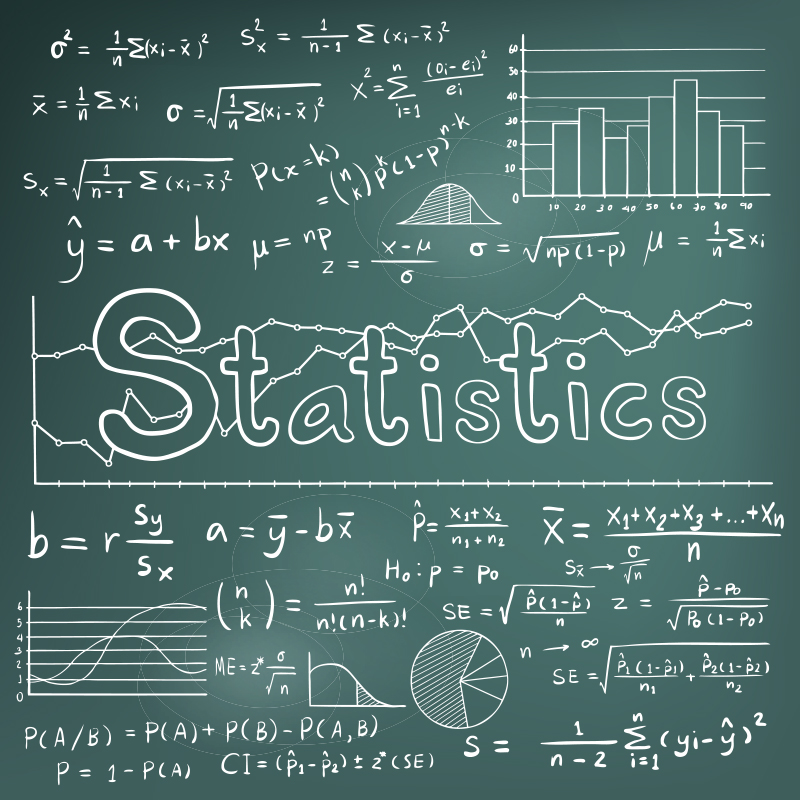
\includegraphics[width=1.0\paperwidth]{statistics-review.jpg}}
  \usebackgroundtemplate{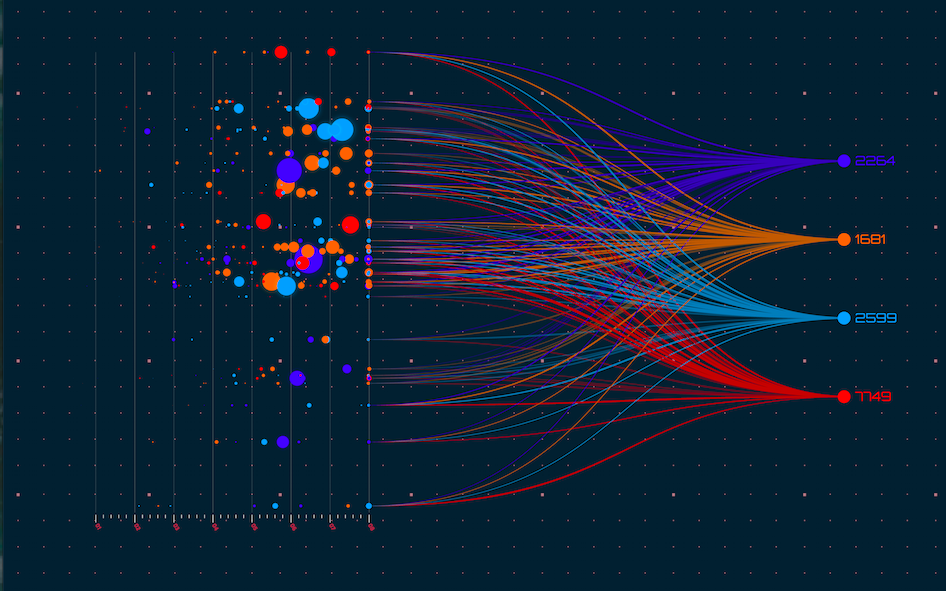
\includegraphics[scale=0.5]{data_via.png}}
  \begin{frame}[plain]
  
\begin{mdframed}[tikzsetting={draw=white,fill=white,fill opacity=0.6,draw opacity=0.4,
               line width=0pt},backgroundcolor=none,leftmargin=20,
               rightmargin=20,innertopmargin=4pt]
\begin{center}
\Huge \textbf{Data Visualization}
\end{center}
\end{mdframed}

  \end{frame}
}

%most reliant on human cognition
%limited only by cognition
%hypothesis generating scheme often functioning as a gateway into more statistical analysis

%@@@@@@@@@@@@@@@@@@@@@@@@@@@@@@@@@@@@@@@@@@@@@@@@@
\begin{frame}
\frametitle{Today:}

\begin{itemize}
\item Introduce some basic data visualizations;
\bigskip
\bigskip
\item Introduce base R graphics API;
\bigskip
\bigskip
\item Exemplars;
\bigskip
\bigskip
\item Chart crimes.
\end{itemize}

\end{frame}

%@@@@@@@@@@@@@@@@@@@@@@@@@@@@@@@@@@@@@@@@@@@@@@@@@
\begin{frame}
\frametitle{Some history...}

\begin{columns}
\begin{column}{0.5\textwidth}
\begin{itemize}
\item Many ways to extract value from data:
\begin{itemize}
\item descriptive statistics;
\item hypothesis testing;
\item simulation;
\item statistical modeling;
\item machine learning/AI;
\end{itemize}
\bigskip
\bigskip
\item One of the very oldest is \textbf{data visualization}:
\begin{itemize}
\item William Playfair often cited as the inventor of line, bar, and pie charts, late 18th century.
\end{itemize}
\end{itemize}

\end{column}
\begin{column}{0.5\textwidth}
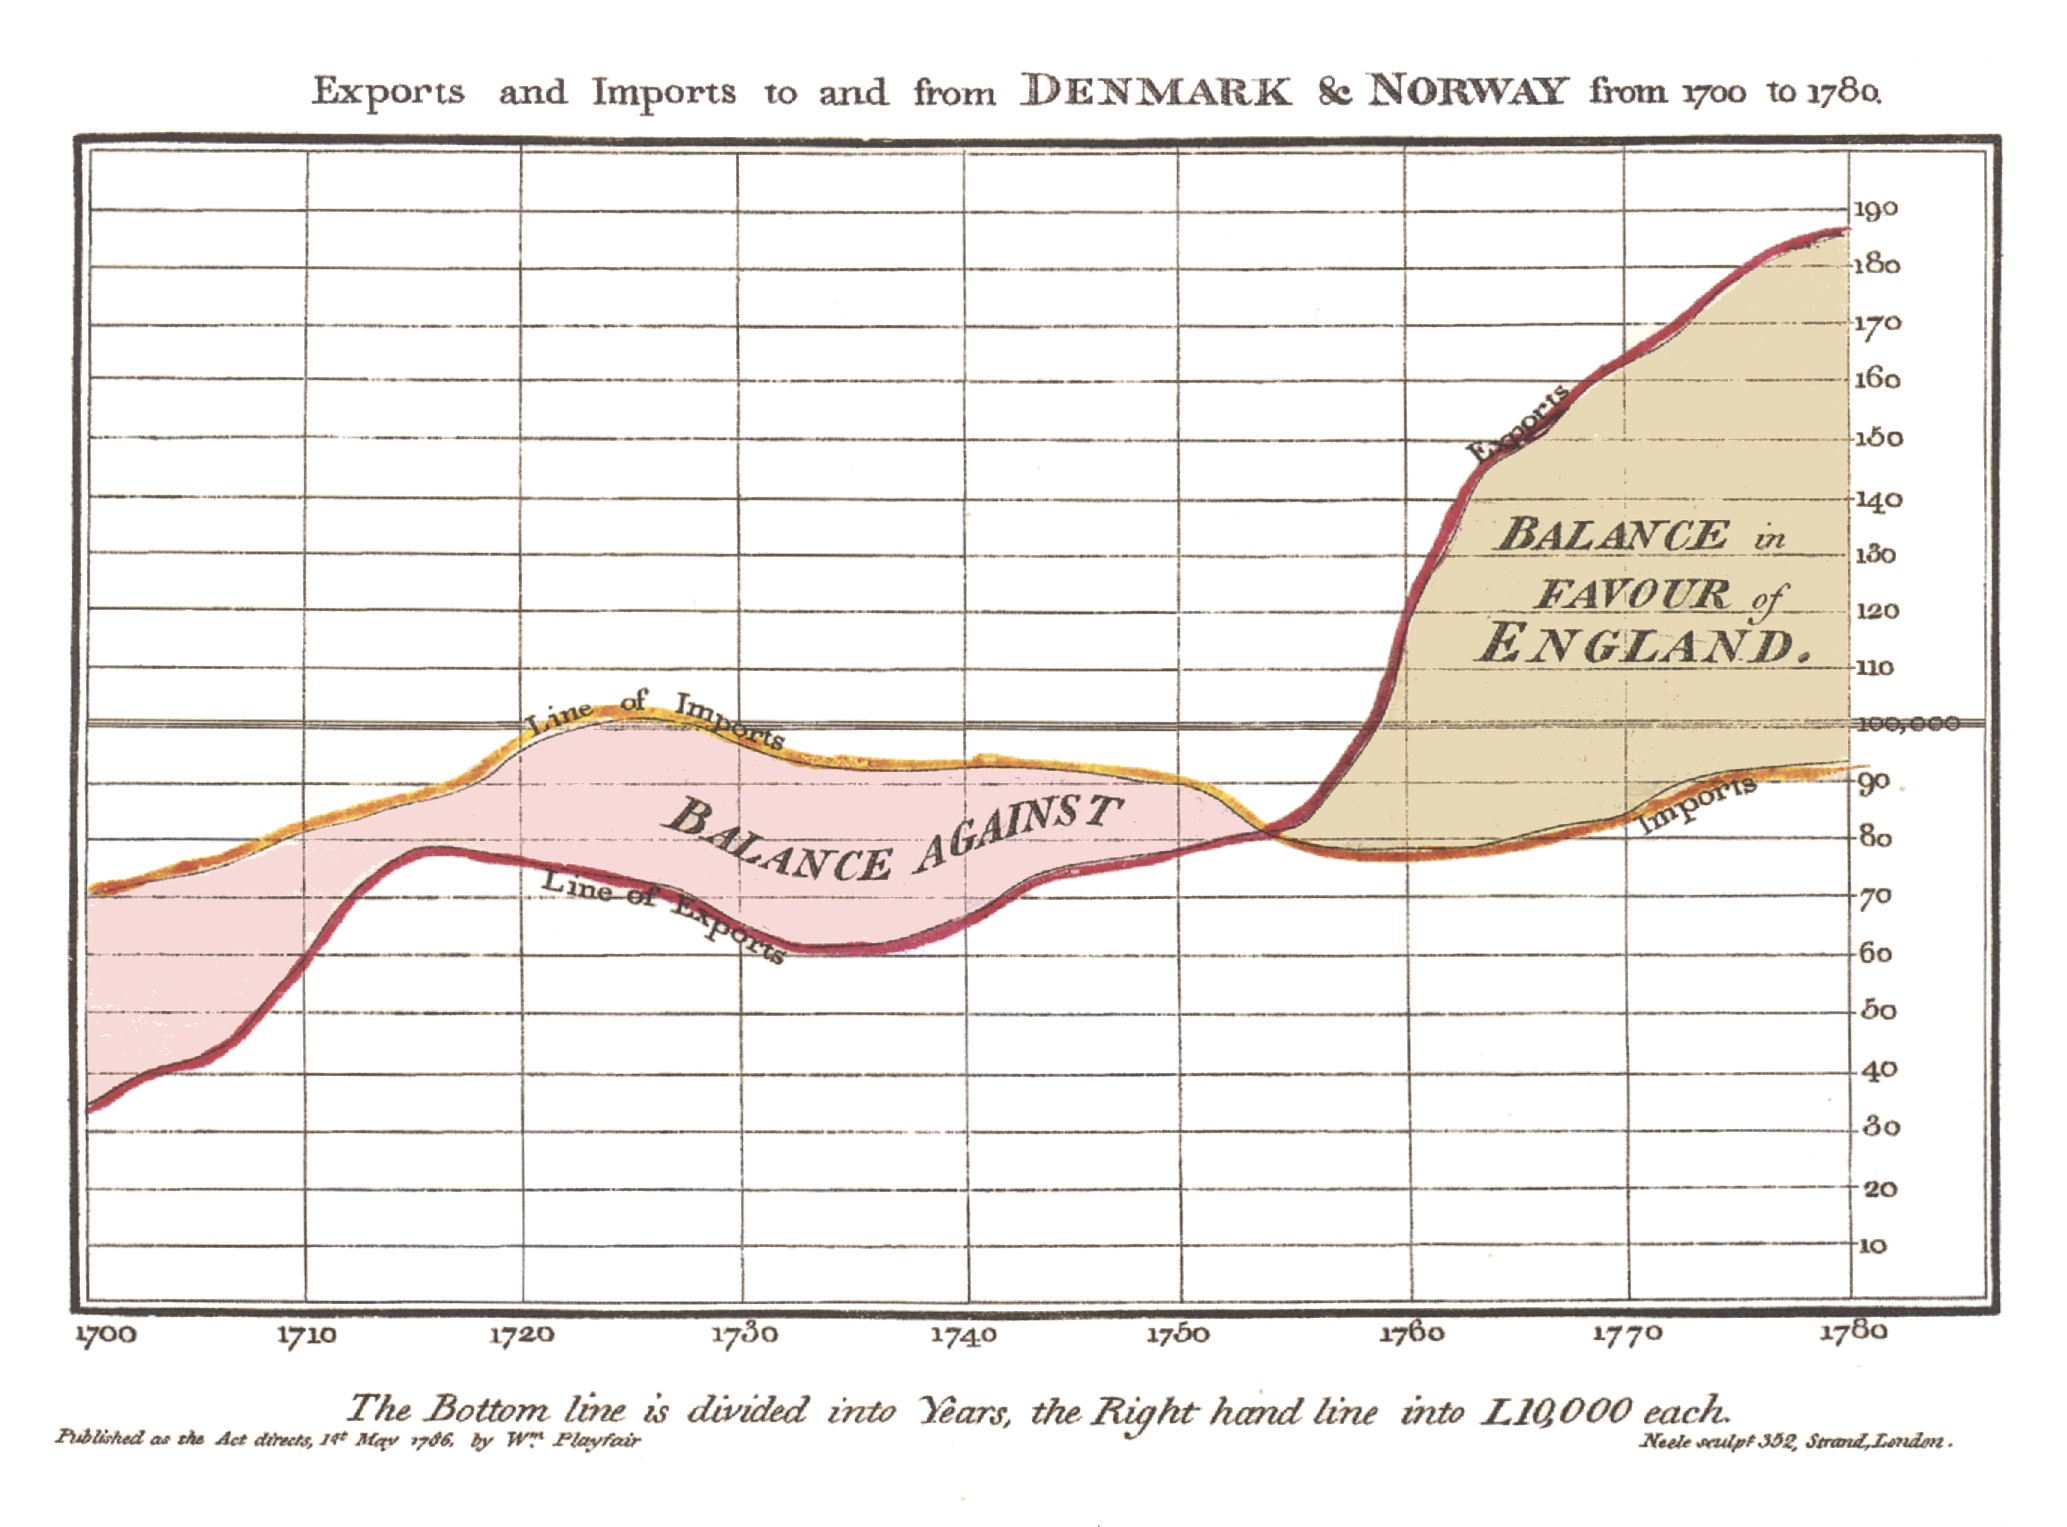
\includegraphics[scale=0.1]{Playfair_TimeSeries-2.png}
\end{column}
\end{columns}

\end{frame}

%@@@@@@@@@@@@@@@@@@@@@@@@@@@@@@@@@@@@@@@@@@@@@@@@@
\begin{frame}
\frametitle{Some history...}

\begin{columns}
\begin{column}{0.5\textwidth}

\begin{itemize}
\item Many ways to extract value from data:
\begin{itemize}
\item descriptive statistics;
\item hypothesis testing;
\item simulation;
\item statistical modeling;
\item machine learning/AI;
\end{itemize}
\bigskip
\bigskip
\item One of the very oldest is \textbf{data visualization}:
\begin{itemize}
\item William Playfair often cited as the inventor of line, bar, and pie charts, late 18th century.
\end{itemize}
\end{itemize}

\end{column}
\begin{column}{0.5\textwidth}
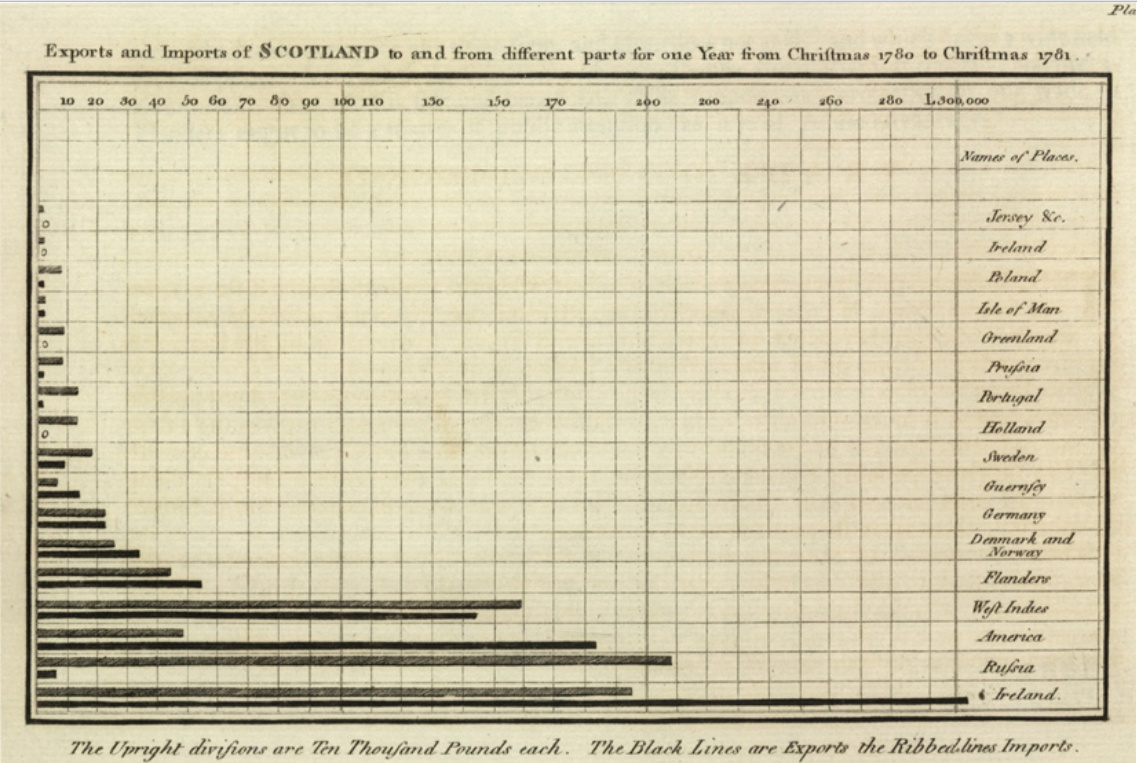
\includegraphics[scale=0.25]{1786_Playfair_-_Exports_and_Imports_of_Scotland_to_and_from_different_parts_for_one_Year_from_Christmas_1780_to_Christmas_1781.jpg}
\end{column}
\end{columns}

\end{frame}

%@@@@@@@@@@@@@@@@@@@@@@@@@@@@@@@@@@@@@@@@@@@@@@@@@
\begin{frame}
\frametitle{Some history...}

\begin{columns}
\begin{column}{0.5\textwidth}

\begin{itemize}
\item Many ways to extract value from data:
\begin{itemize}
\item descriptive statistics;
\item hypothesis testing;
\item simulation;
\item statistical modeling;
\item machine learning/AI;
\end{itemize}
\bigskip
\bigskip
\item One of the very oldest is \textbf{data visualization}:
\begin{itemize}
\item William Playfair often cited as the inventor of line, bar, and pie charts, late 18th century.
\end{itemize}
\end{itemize}

\end{column}
\begin{column}{0.5\textwidth}
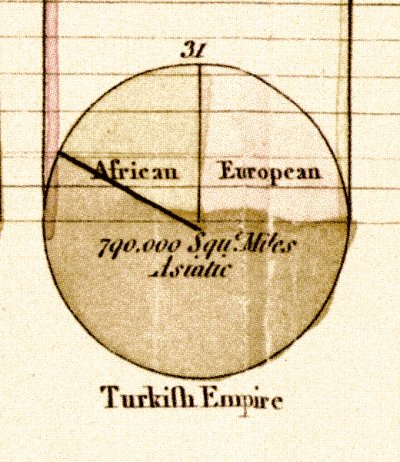
\includegraphics[scale=2.6]{Playfair-piechart.jpg}
\end{column}
\end{columns}

\end{frame}

%@@@@@@@@@@@@@@@@@@@@@@@@@@@@@@@@@@@@@@@@@@@@@@@@@
\begin{frame}
\frametitle{Goals:}
\begin{itemize}
\item Characteristics of data visualization:
\begin{itemize}
\item Data encoded as a visual object;
\item Goal of any data analysis is to help audience reason about the data -- data viz is most reliant on human cognition for inference and meaning;
\item Form $=$ substance;
\item Generally, necessarily low dimensional;
\end{itemize}
\bigskip
\item Data visualization should (Tufte 1983):
\begin{itemize}
\item Have message fit for audience purpose and communicate information;
\item Highlight the data;
\item Help the audience focus on the substance;
\item NOT distort the data or knowingly perpetuate a lie;
\item Put many numbers in a small, accessible space;
\item Enable the audience to grapple with large data sets coherently;
\item Encourage viewers to compare data effectively;
\item Allow investigation of both micro and macro level structure in the data; 
\item integrate closely with additional statistical analysis.
\end{itemize}
\end{itemize}
\end{frame}

%@@@@@@@@@@@@@@@@@@@@@@@@@@@@@@@@@@@@@@@@@@@@@@@@@
\begin{frame}
\frametitle{Some of my favorite types of graphics}


\begin{columns}
\begin{column}{0.5\textwidth}

\begin{itemize}
\item \textbf{Bar chart};
\begin{itemize}
\item Compare amount in fixed bins;
\item Used for \textbf{categorical} data where there is no order;
\end{itemize}


\item \textbf{Histogram};
\begin{itemize}
\item Compare amount in constructed bins;
\item Used for \textbf{continuous} data;
\end{itemize}


\item \textbf{Density plot};
\begin{itemize}
\item Smoothed comparison of amount in constructed bins;
\item Used for \textbf{continuous} data;
\end{itemize}


\item \textbf{Scatterplot};
\begin{itemize}
\item Compare two variables;
\item Used for $\mathbf{(x,y)}$ data;
\end{itemize}

\end{itemize}

\end{column}

\begin{column}{0.5\textwidth}
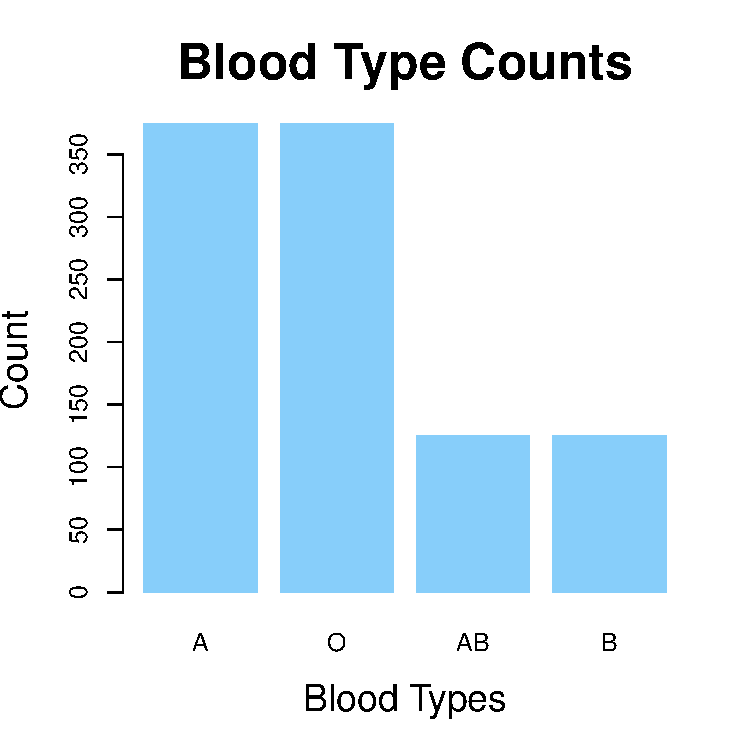
\includegraphics[scale=0.5]{bar_chart.pdf}
\end{column}

\end{columns}

\end{frame}

%@@@@@@@@@@@@@@@@@@@@@@@@@@@@@@@@@@@@@@@@@@@@@@@@@
\begin{frame}
\frametitle{Some of my favorite types of graphics}


\begin{columns}
\begin{column}{0.5\textwidth}

\begin{itemize}
\item \textbf{Bar chart};
\begin{itemize}
\item Compare amount in fixed bins;
\item Used for \textbf{categorical} data where there is no order;
\end{itemize}


\item \textbf{Histogram};
\begin{itemize}
\item Compare amount in constructed bins;
\item Used for \textbf{continuous} data;
\end{itemize}


\item \textbf{Density plot};
\begin{itemize}
\item Smoothed comparison of amount in constructed bins;
\item Used for \textbf{continuous} data;
\end{itemize}


\item \textbf{Scatterplot};
\begin{itemize}
\item Compare two variables;
\item Used for $\mathbf{(x,y)}$ data;
\end{itemize}

\end{itemize}

\end{column}

\begin{column}{0.5\textwidth}
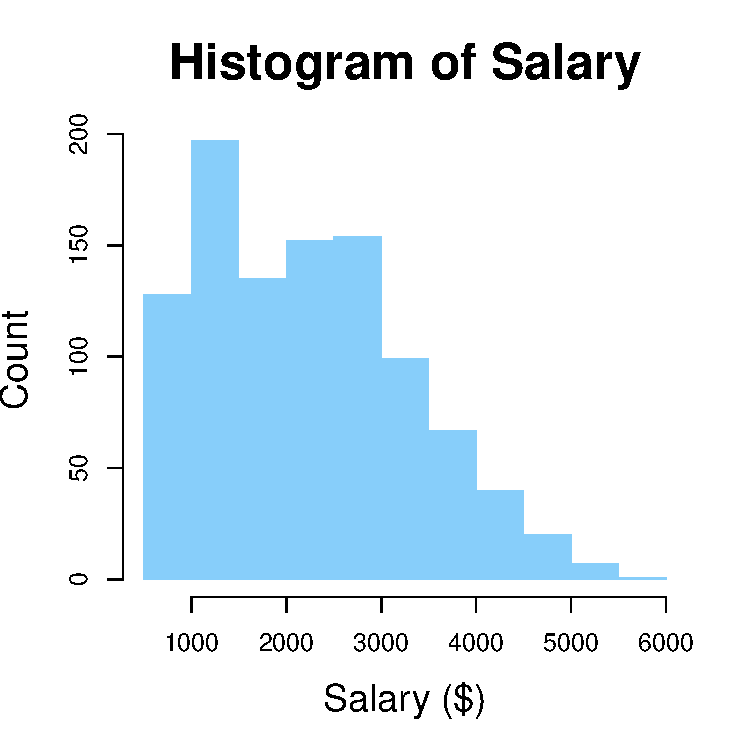
\includegraphics[scale=0.5]{histogram_10.pdf}
\end{column}

\end{columns}

\end{frame}

%@@@@@@@@@@@@@@@@@@@@@@@@@@@@@@@@@@@@@@@@@@@@@@@@@
\begin{frame}
\frametitle{Some of my favorite types of graphics}


\begin{columns}
\begin{column}{0.5\textwidth}

\begin{itemize}
\item \textbf{Bar chart};
\begin{itemize}
\item Compare amount in fixed bins;
\item Used for \textbf{categorical} data where there is no order;
\end{itemize}


\item \textbf{Histogram};
\begin{itemize}
\item Compare amount in constructed bins;
\item Used for \textbf{continuous} data;
\end{itemize}


\item \textbf{Density plot};
\begin{itemize}
\item Smoothed comparison of amount in constructed bins;
\item Used for \textbf{continuous} data;
\end{itemize}


\item \textbf{Scatterplot};
\begin{itemize}
\item Compare two variables;
\item Used for $\mathbf{(x,y)}$ data;
\end{itemize}

\end{itemize}

\end{column}

\begin{column}{0.5\textwidth}
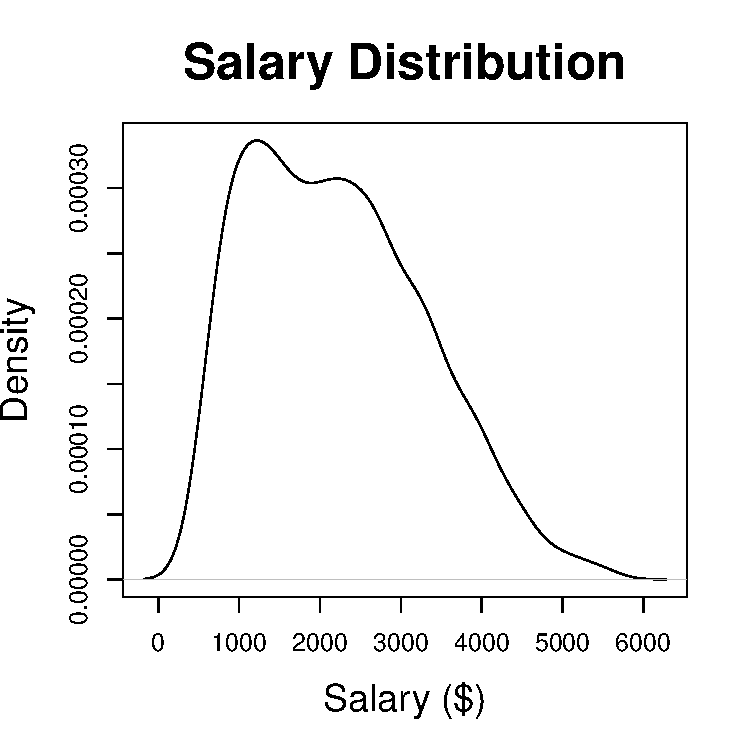
\includegraphics[scale=0.5]{salary_distribution.pdf}
\end{column}

\end{columns}

\end{frame}

%@@@@@@@@@@@@@@@@@@@@@@@@@@@@@@@@@@@@@@@@@@@@@@@@@
\begin{frame}
\frametitle{Some of my favorite types of graphics}


\begin{columns}
\begin{column}{0.5\textwidth}

\begin{itemize}
\item \textbf{Bar chart};
\begin{itemize}
\item Compare amount in fixed bins;
\item Used for \textbf{categorical} data where there is no order;
\end{itemize}


\item \textbf{Histogram};
\begin{itemize}
\item Compare amount in constructed bins;
\item Used for \textbf{continuous} data;
\end{itemize}


\item \textbf{Density plot};
\begin{itemize}
\item Smoothed comparison of amount in constructed bins;
\item Used for \textbf{continuous} data;
\end{itemize}


\item \textbf{Scatterplot};
\begin{itemize}
\item Compare two variables;
\item Used for $\mathbf{(x,y)}$ data;
\end{itemize}

\end{itemize}

\end{column}

\begin{column}{0.5\textwidth}
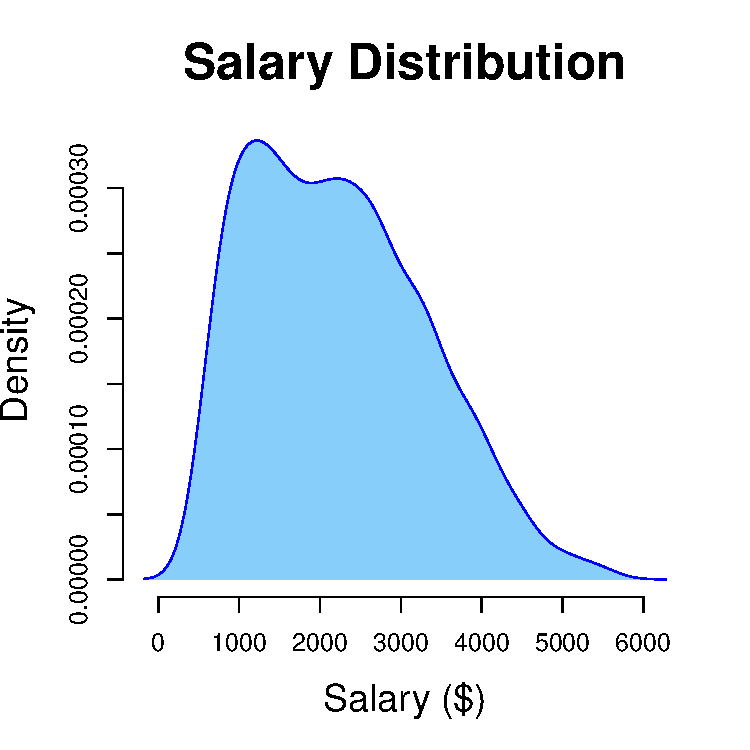
\includegraphics[scale=0.5]{salary_distribution_fancy.pdf}
\end{column}

\end{columns}

\end{frame}

%@@@@@@@@@@@@@@@@@@@@@@@@@@@@@@@@@@@@@@@@@@@@@@@@@
\begin{frame}
\frametitle{Some of my favorite types of graphics}


\begin{columns}
\begin{column}{0.5\textwidth}

\begin{itemize}
\item \textbf{Bar chart};
\begin{itemize}
\item Compare amount in fixed bins;
\item Used for \textbf{categorical} data where there is no order;
\end{itemize}


\item \textbf{Histogram};
\begin{itemize}
\item Compare amount in constructed bins;
\item Used for \textbf{continuous} data;
\end{itemize}


\item \textbf{Density plot};
\begin{itemize}
\item Smoothed comparison of amount in constructed bins;
\item Used for \textbf{continuous} data;
\end{itemize}


\item \textbf{Scatterplot};
\begin{itemize}
\item Compare two variables;
\item Used for $\mathbf{(x,y)}$ data;
\end{itemize}

\end{itemize}

\end{column}

\begin{column}{0.5\textwidth}
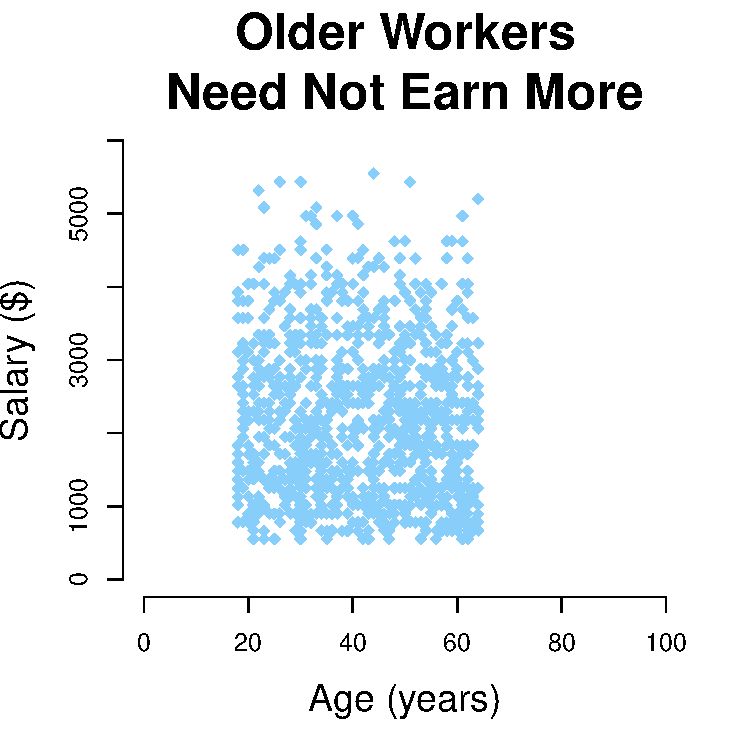
\includegraphics[scale=0.5]{age_v_salary.pdf}
\end{column}

\end{columns}

\end{frame}

%%@@@@@@@@@@@@@@@@@@@@@@@@@@@@@@@@@@@@@@@@@@@@@@@@@
%\begin{frame}
%\frametitle{Connections}
%\begin{center}
%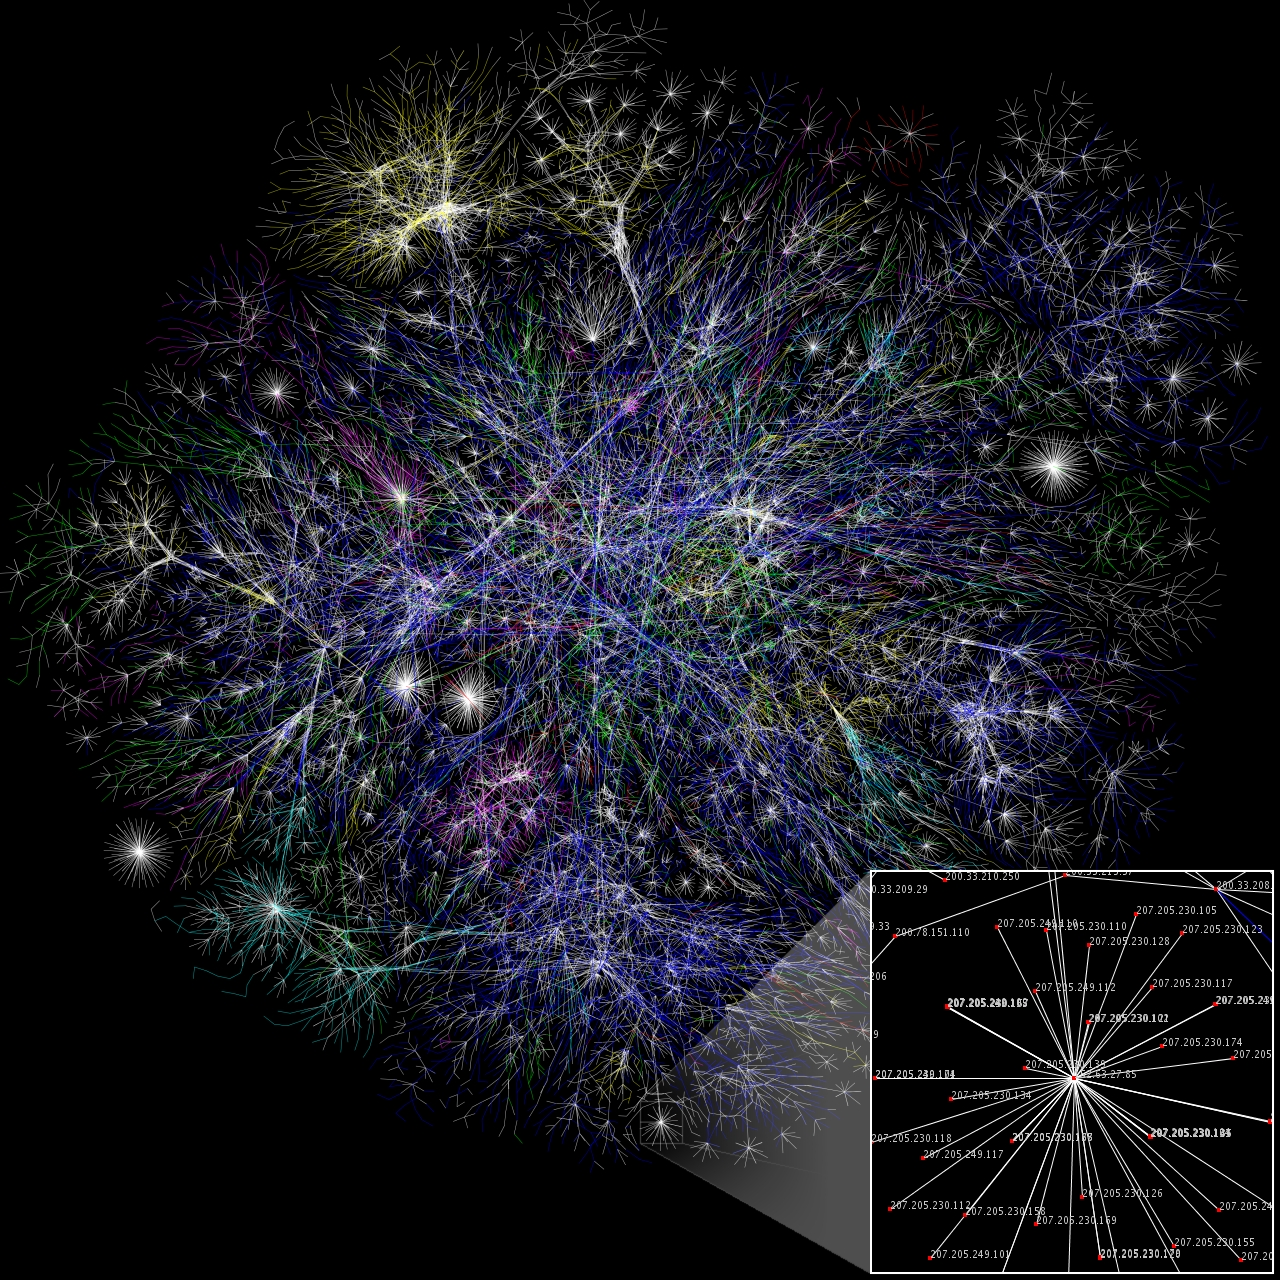
\includegraphics[scale=0.17]{Internet_map_2005.jpg}
%\end{center}
%
%\end{frame}
%
%%@@@@@@@@@@@@@@@@@@@@@@@@@@@@@@@@@@@@@@@@@@@@@@@@@
%\begin{frame}
%\frametitle{Connections: dimensions of information}
%
%\begin{itemize}
%\item Number of internet locations (IP addresses);
%\bigskip
%\bigskip
%\item Links between different locations;
%\bigskip
%\bigskip
%\item Location in `internet space';
%\end{itemize}
%
%\end{frame}

%@@@@@@@@@@@@@@@@@@@@@@@@@@@@@@@@@@@@@@@@@@@@@@@@@
\begin{frame}
\frametitle{Congressional Partisanship}
\begin{center}
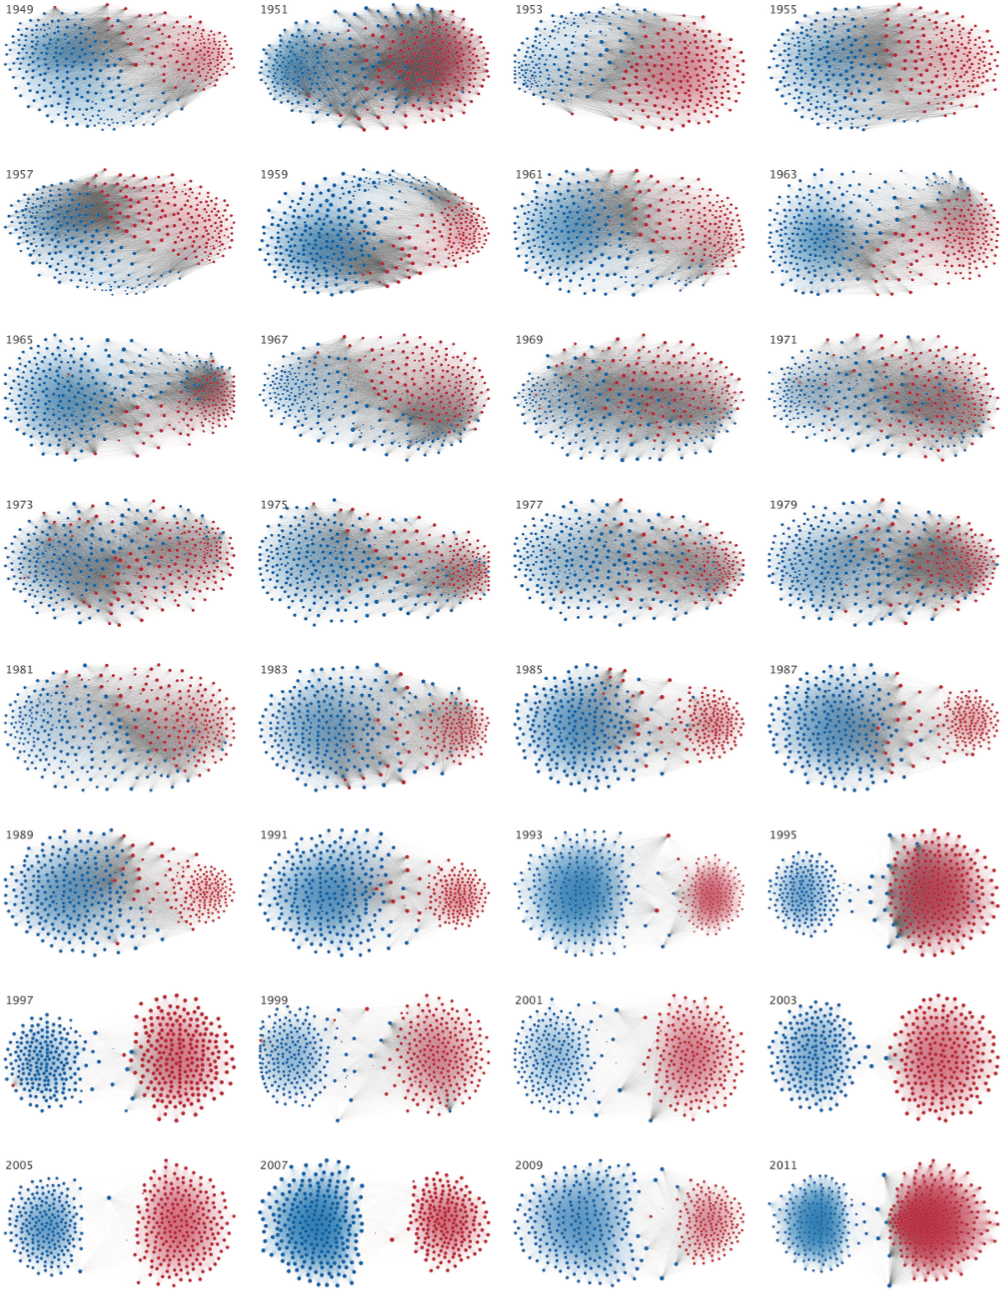
\includegraphics[scale=0.7]{congress_partisanship.png}
\end{center}

\end{frame}

%@@@@@@@@@@@@@@@@@@@@@@@@@@@@@@@@@@@@@@@@@@@@@@@@@
\begin{frame}
\frametitle{Congressional Partisanship: dimensions of information}

\begin{itemize}
\item Number of legislators;
\bigskip
\item Party identification;
\bigskip
\item Legislator location in `ideological space';
\bigskip
\item Number of vote associations between legislators;
\bigskip
\item Time in years.
\end{itemize}

\end{frame}

%@@@@@@@@@@@@@@@@@@@@@@@@@@@@@@@@@@@@@@@@@@@@@@@@@
\begin{frame}
\frametitle{Makeup of Congress}
\begin{center}
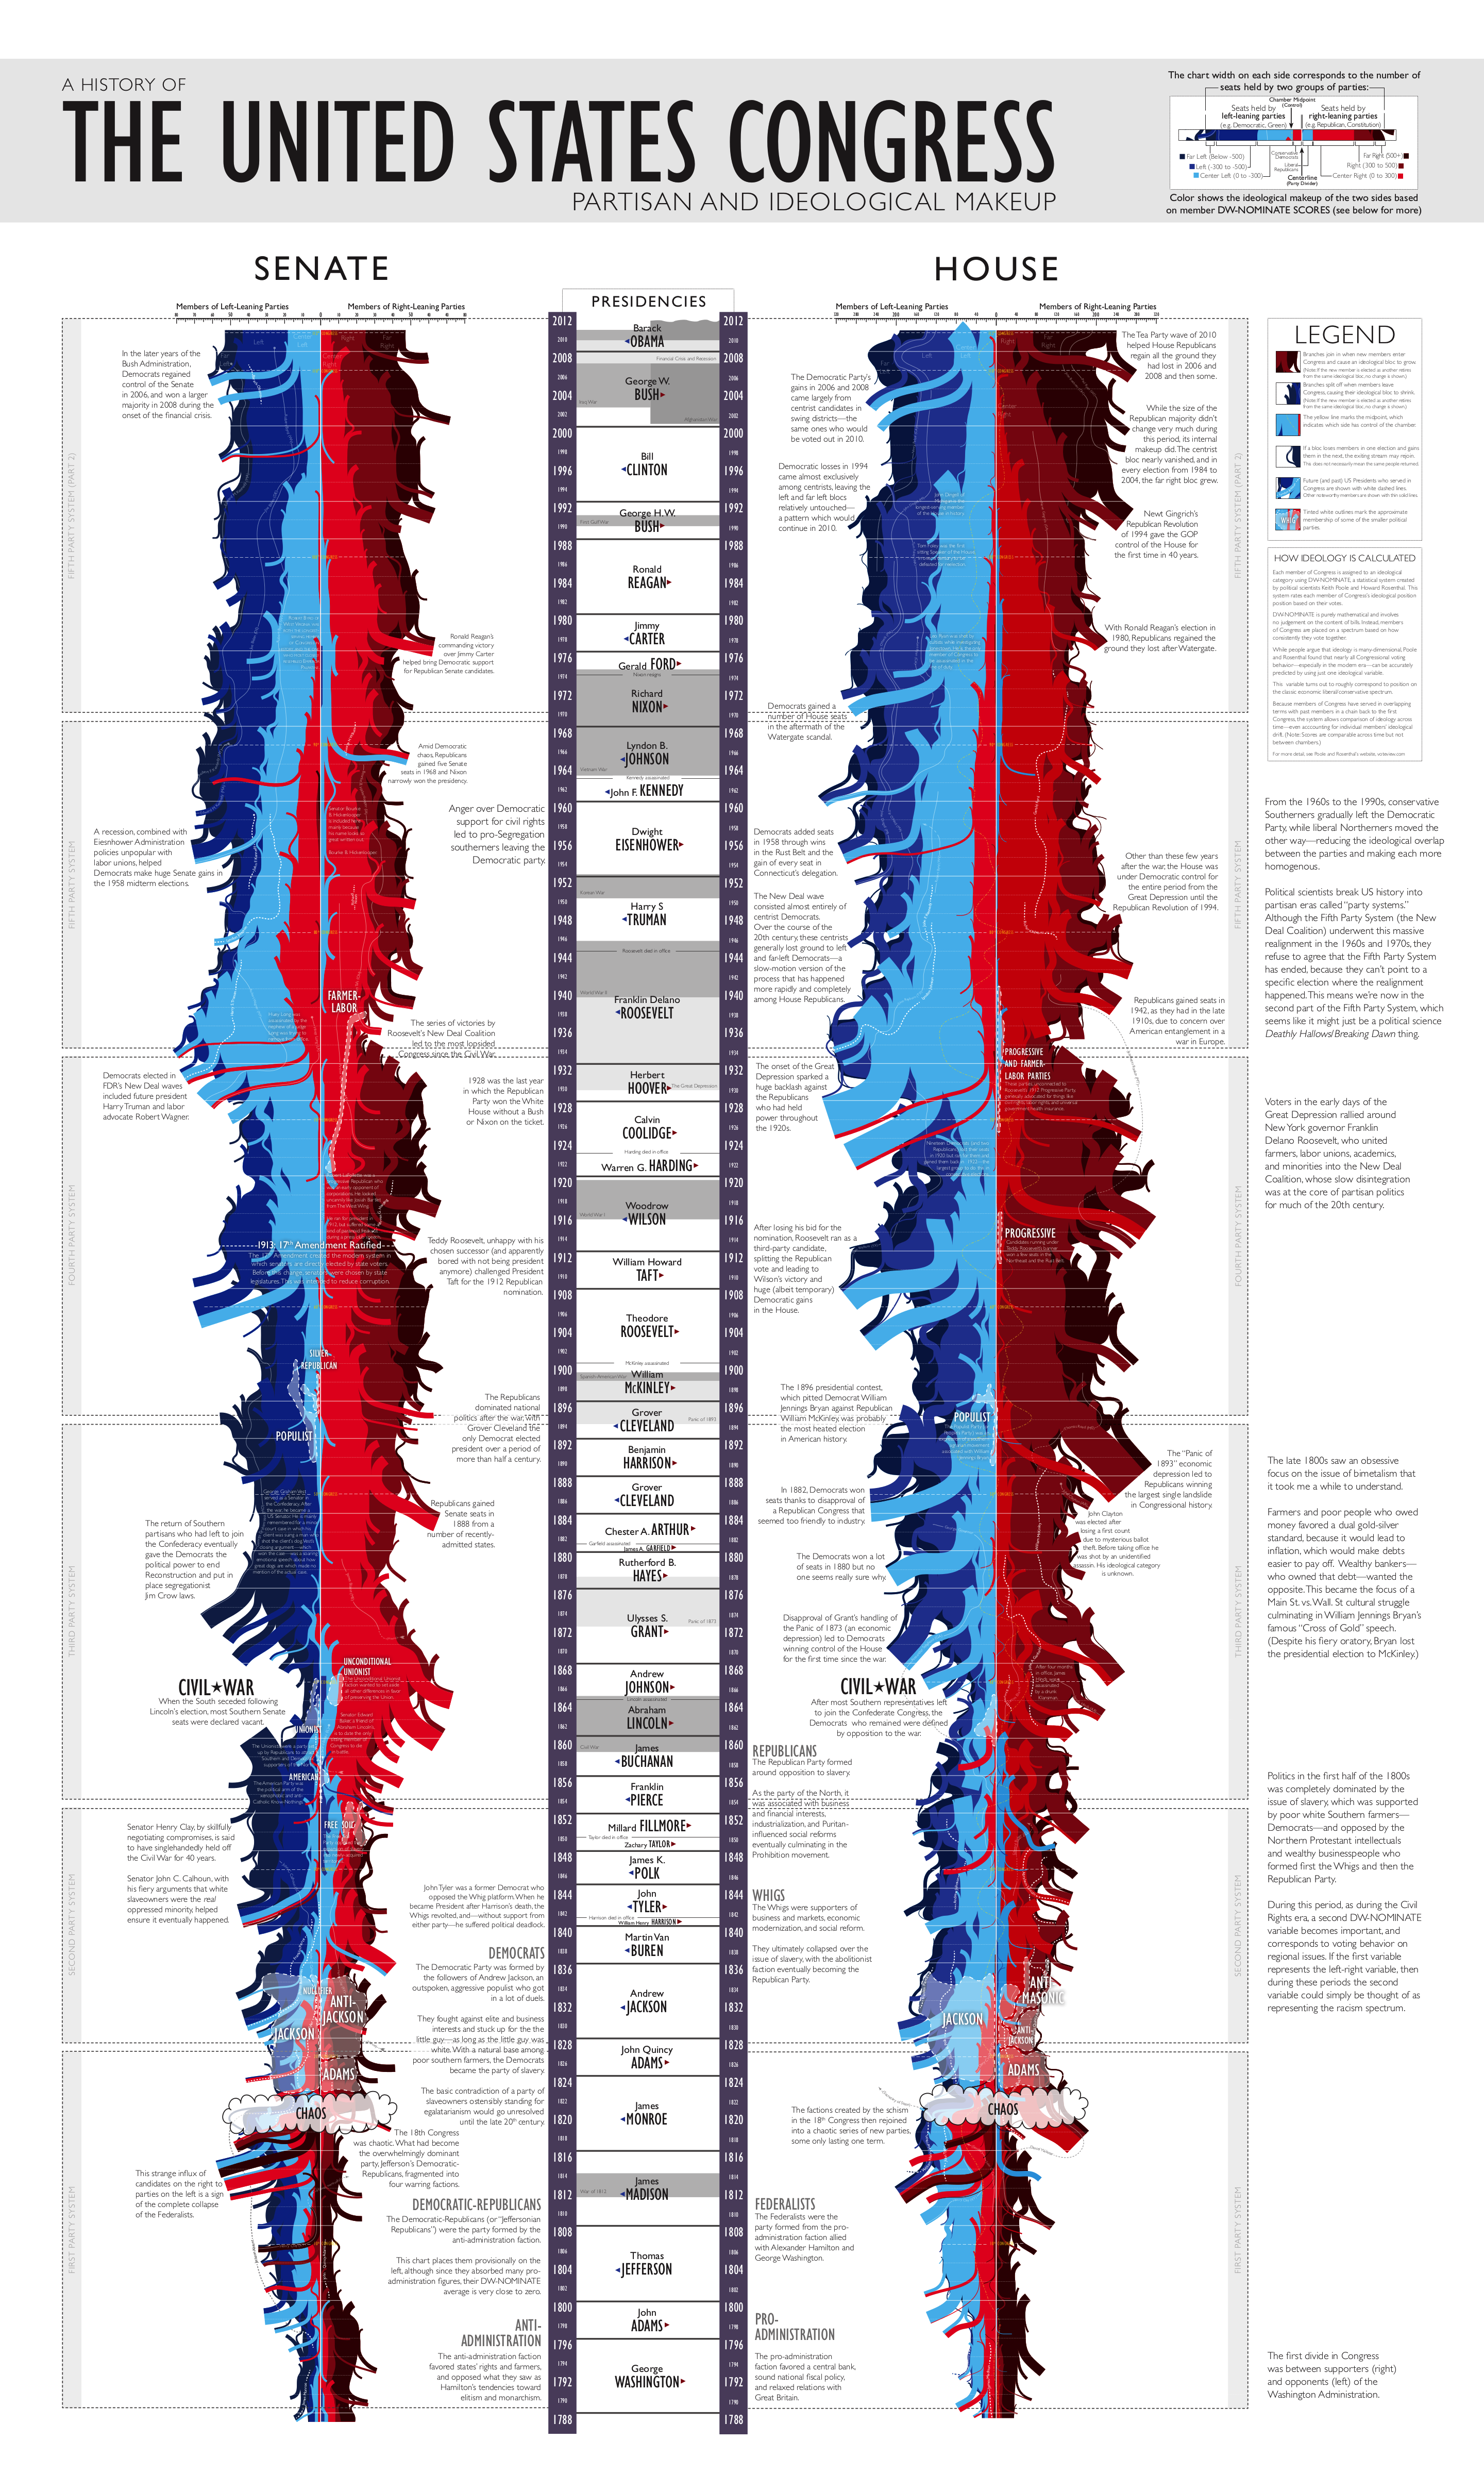
\includegraphics[scale=0.2]{congress_large.png}
\end{center}

\end{frame}

%@@@@@@@@@@@@@@@@@@@@@@@@@@@@@@@@@@@@@@@@@@@@@@@@@
\begin{frame}
\frametitle{Makeup of Congress}
\begin{center}
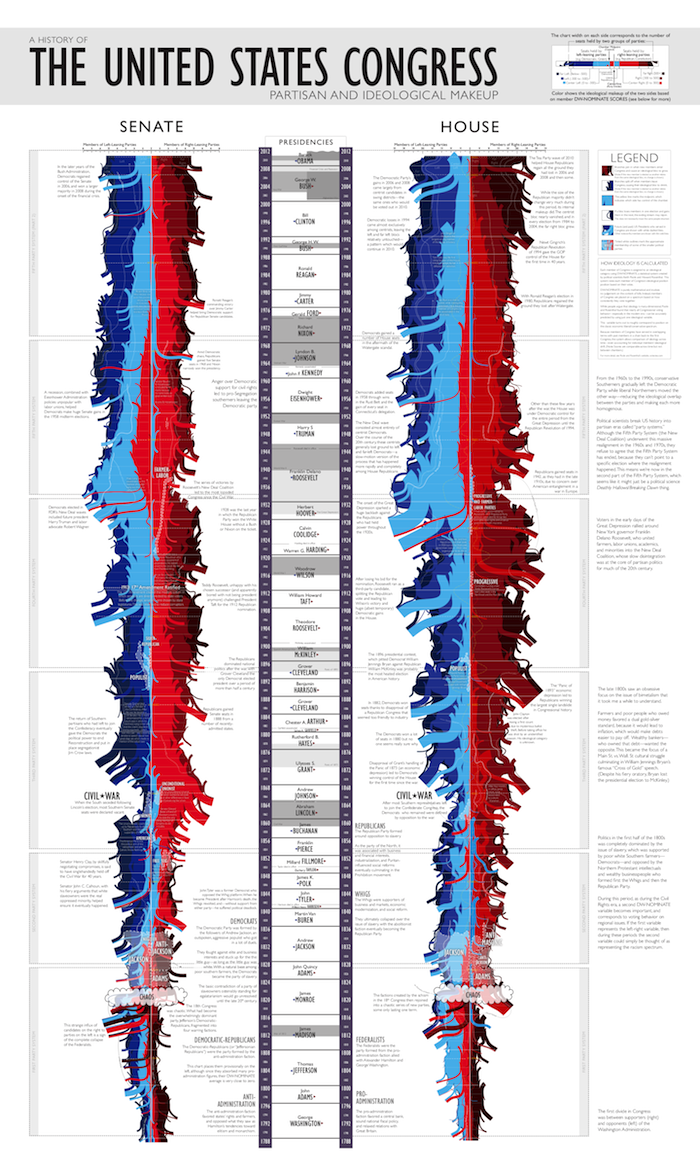
\includegraphics[scale=0.18]{congress.png}
\end{center}

\end{frame}

%@@@@@@@@@@@@@@@@@@@@@@@@@@@@@@@@@@@@@@@@@@@@@@@@@
\begin{frame}
\frametitle{Makeup of Congress: dimensions of information}

\begin{itemize}
\item Number of legislators;
\bigskip
\item Size of parties in congress;
\bigskip
\item Size of congress itself;
\bigskip
\item Size of intra-party ideological blocks;
\bigskip
\item Block entry/exit;
\bigskip
\item Time in years.
\end{itemize}

\end{frame}

%@@@@@@@@@@@@@@@@@@@@@@@@@@@@@@@@@@@@@@@@@@@@@@@@@
\begin{frame}
\frametitle{Napoleon's Progress}
\begin{center}
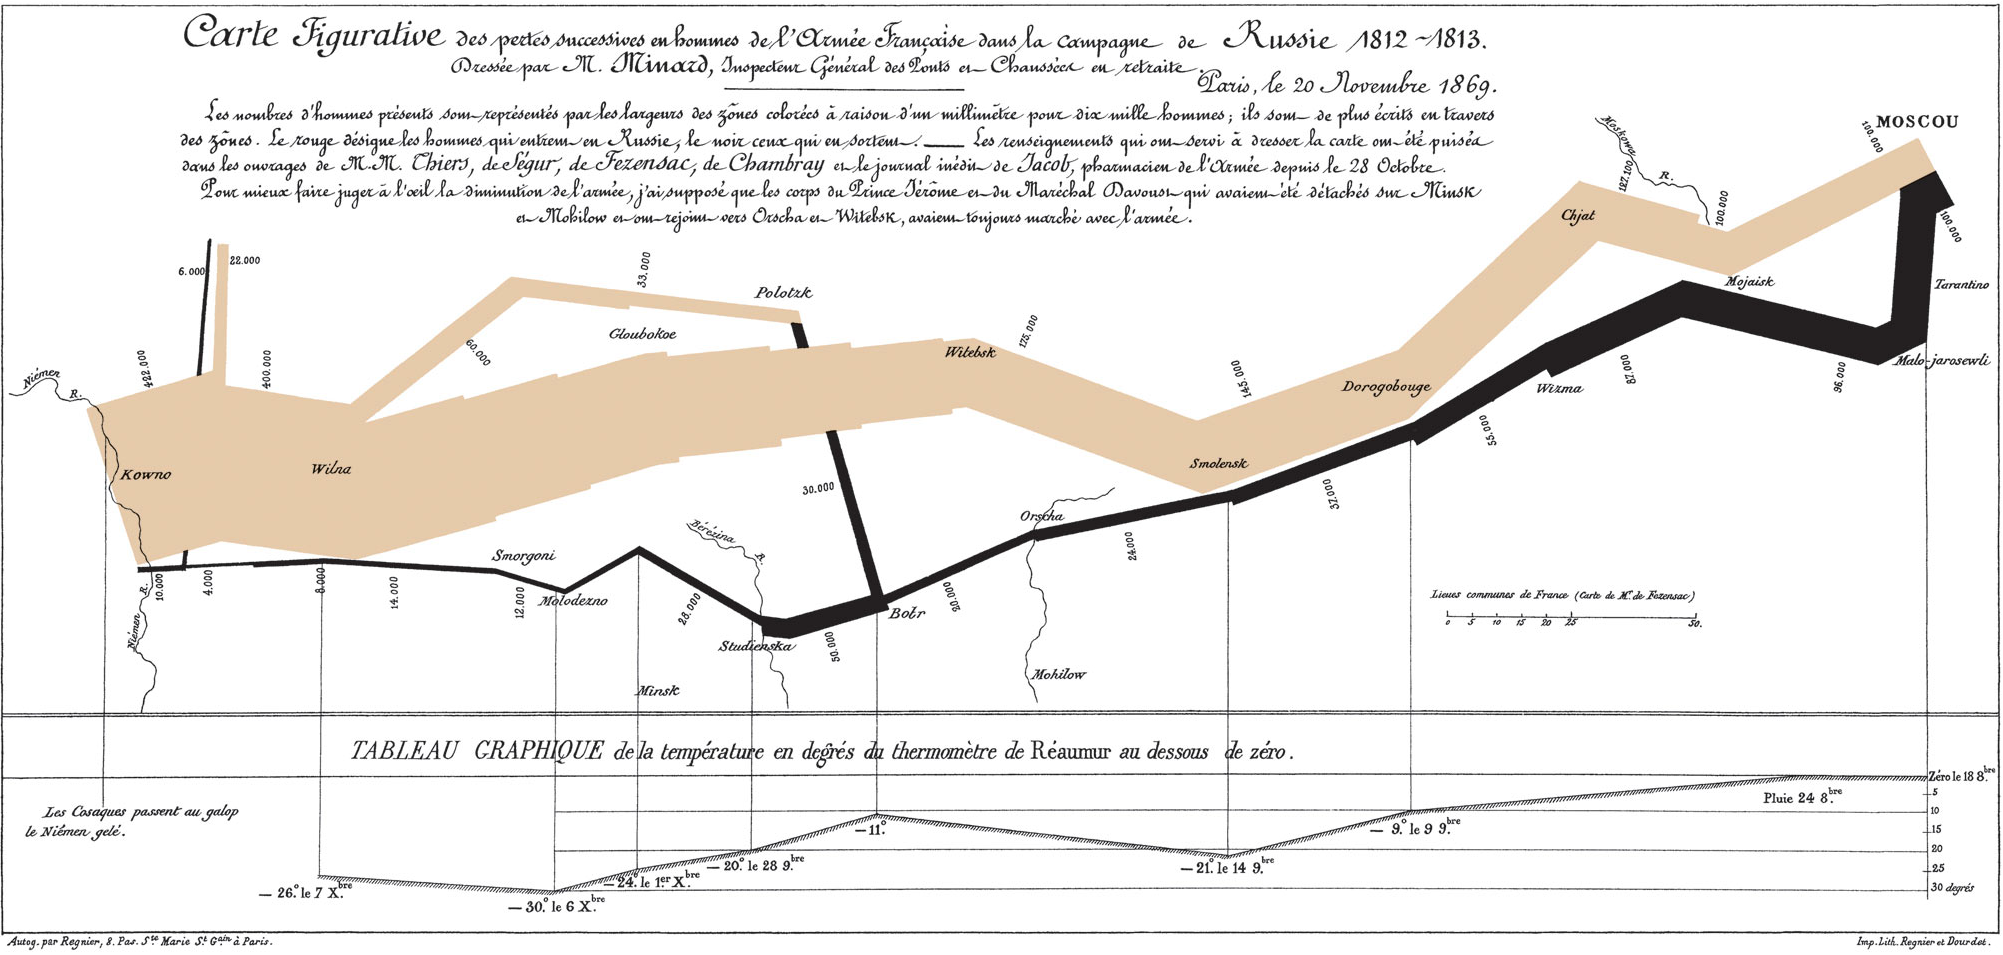
\includegraphics[scale=0.28]{Minard.png}
\end{center}

\end{frame}

%@@@@@@@@@@@@@@@@@@@@@@@@@@@@@@@@@@@@@@@@@@@@@@@@@
\begin{frame}
\frametitle{Napoleon's Progress: dimensions of information}

\begin{itemize}
\item Distance traveled by French Army;
\bigskip
\item Geographic location in terms of latitude and longitude;
\bigskip
\item Number of soldiers capable of fighting in French Army -- relative to beginning of campaign;
\bigskip
\item French army advancing or retreating?
\bigskip
\item Time of year;
\bigskip
\item Temperature.
\end{itemize}

\end{frame}

%@@@@@@@@@@@@@@@@@@@@@@@@@@@@@@@@@@@@@@@@@@@@@@@@@
\begin{frame}
\frametitle{Dynamics in Afghanistan}
\begin{center}
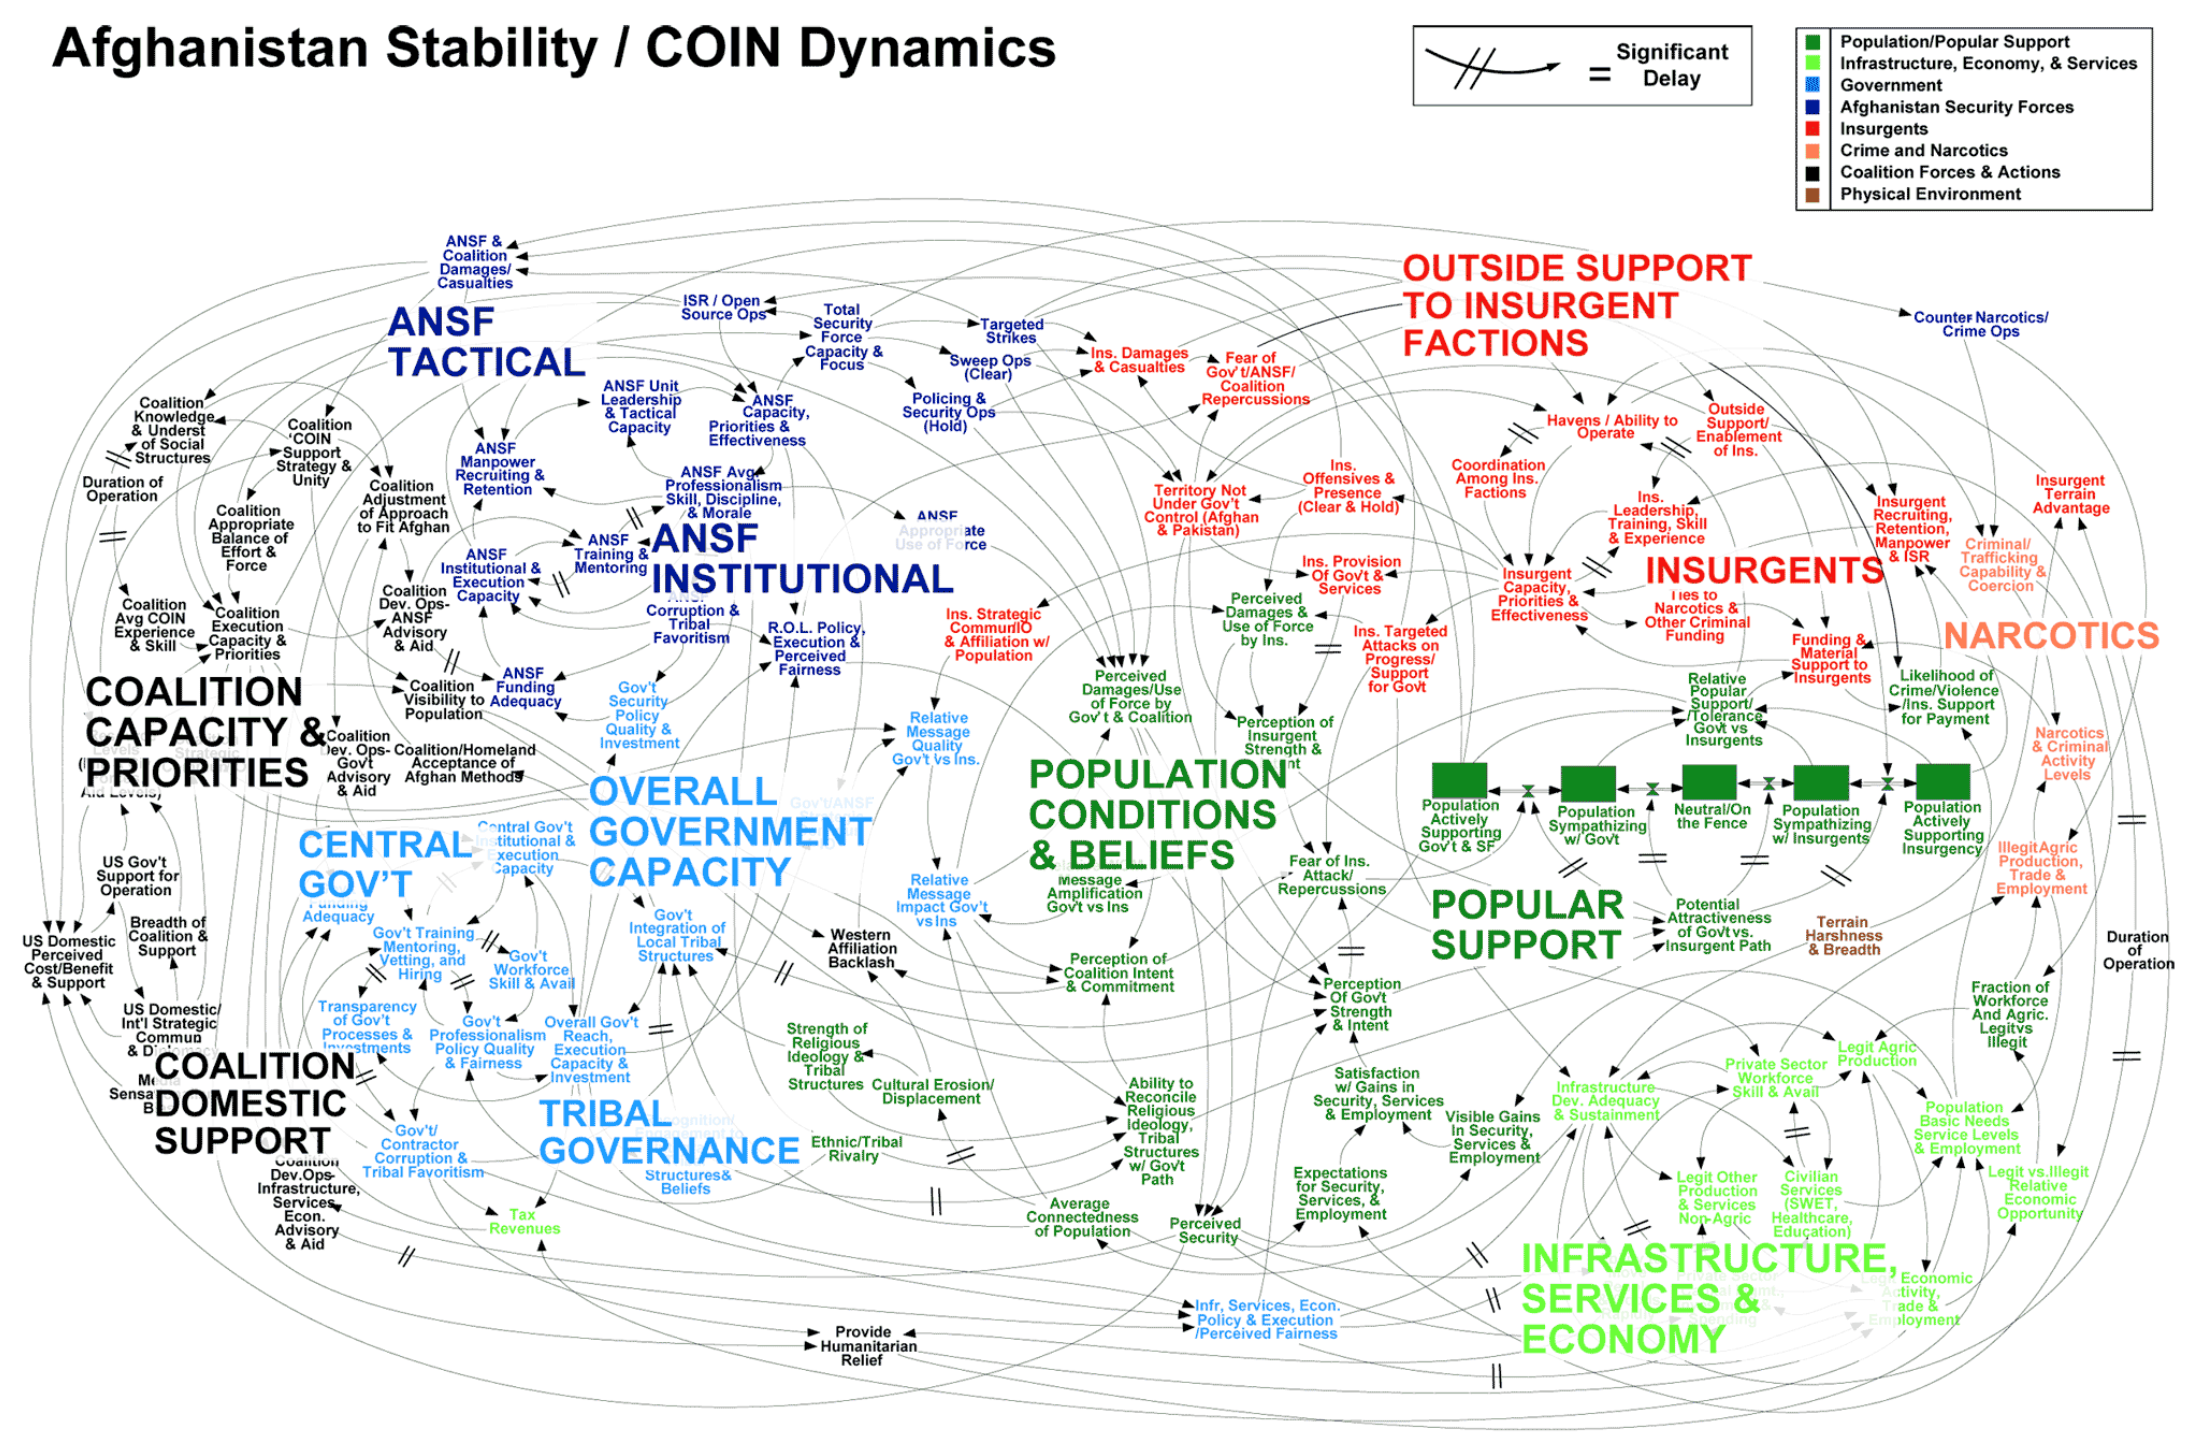
\includegraphics[scale=0.28]{afghan_coin.png}
\end{center}

\end{frame}

%@@@@@@@@@@@@@@@@@@@@@@@@@@@@@@@@@@@@@@@@@@@@@@@@@
\begin{frame}
\frametitle{Chart Crime:}

\begin{center}
\huge \textbf{Impossible to focus.}
\end{center}

\end{frame}

%@@@@@@@@@@@@@@@@@@@@@@@@@@@@@@@@@@@@@@@@@@@@@@@@@
\begin{frame}
\frametitle{COVID Timeline}
\begin{center}
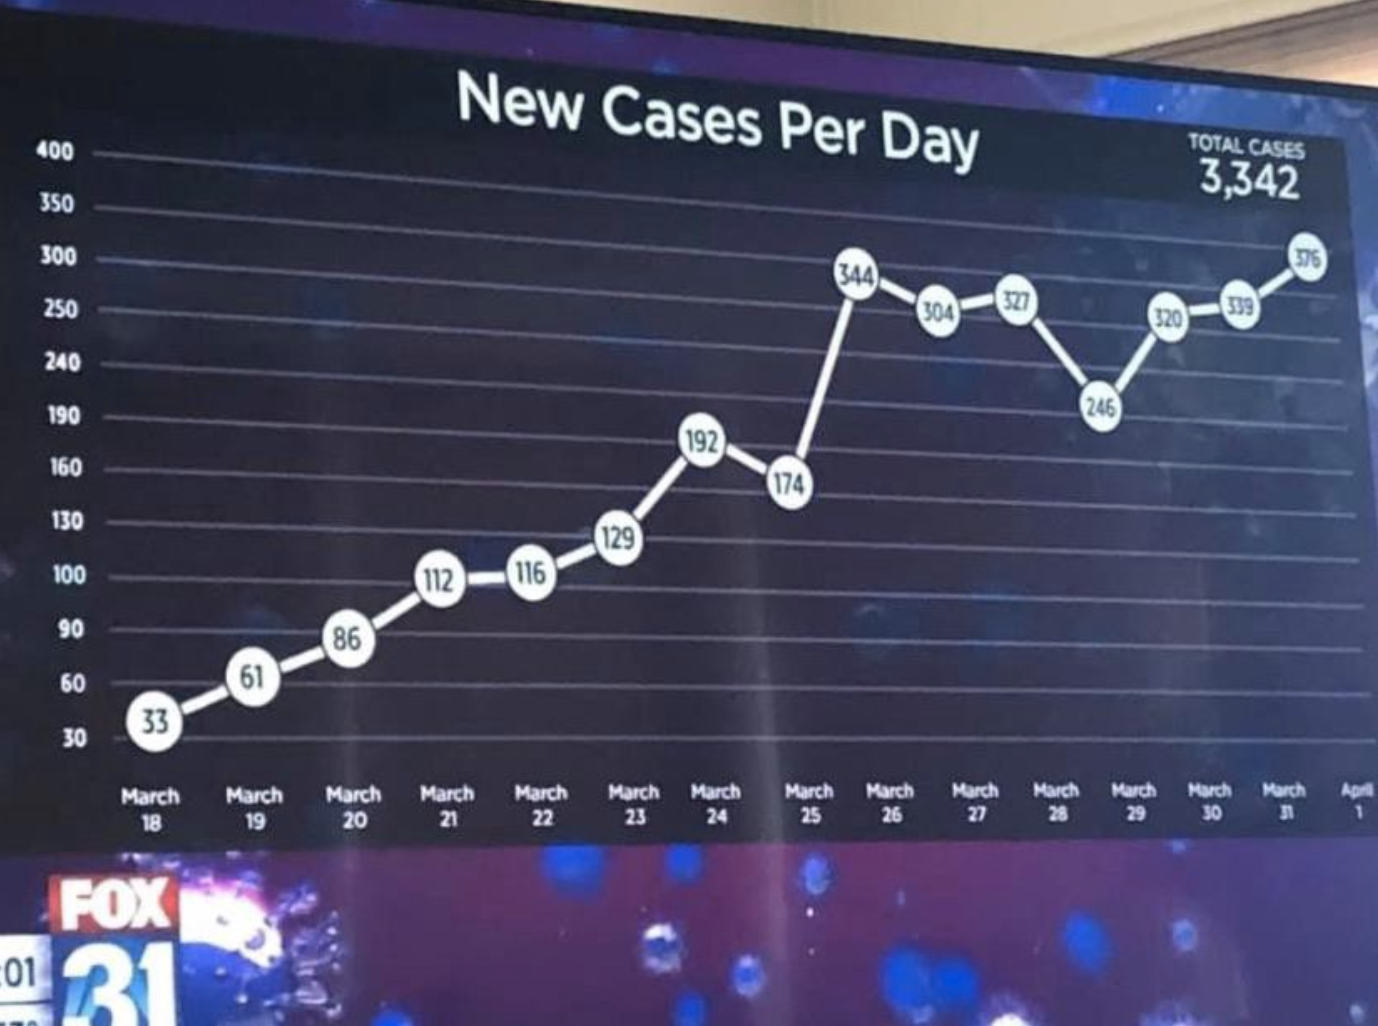
\includegraphics[scale=0.4]{bs_nonlinear_y_axis.png}
\end{center}

\end{frame}

%@@@@@@@@@@@@@@@@@@@@@@@@@@@@@@@@@@@@@@@@@@@@@@@@@
\begin{frame}
\frametitle{Chart Crime:}

\begin{center}
\huge \textbf{Non-linear $y$-axis.}
\end{center}

\end{frame}

%@@@@@@@@@@@@@@@@@@@@@@@@@@@@@@@@@@@@@@@@@@@@@@@@@
\begin{frame}
\frametitle{COVID's Reach}
\begin{center}
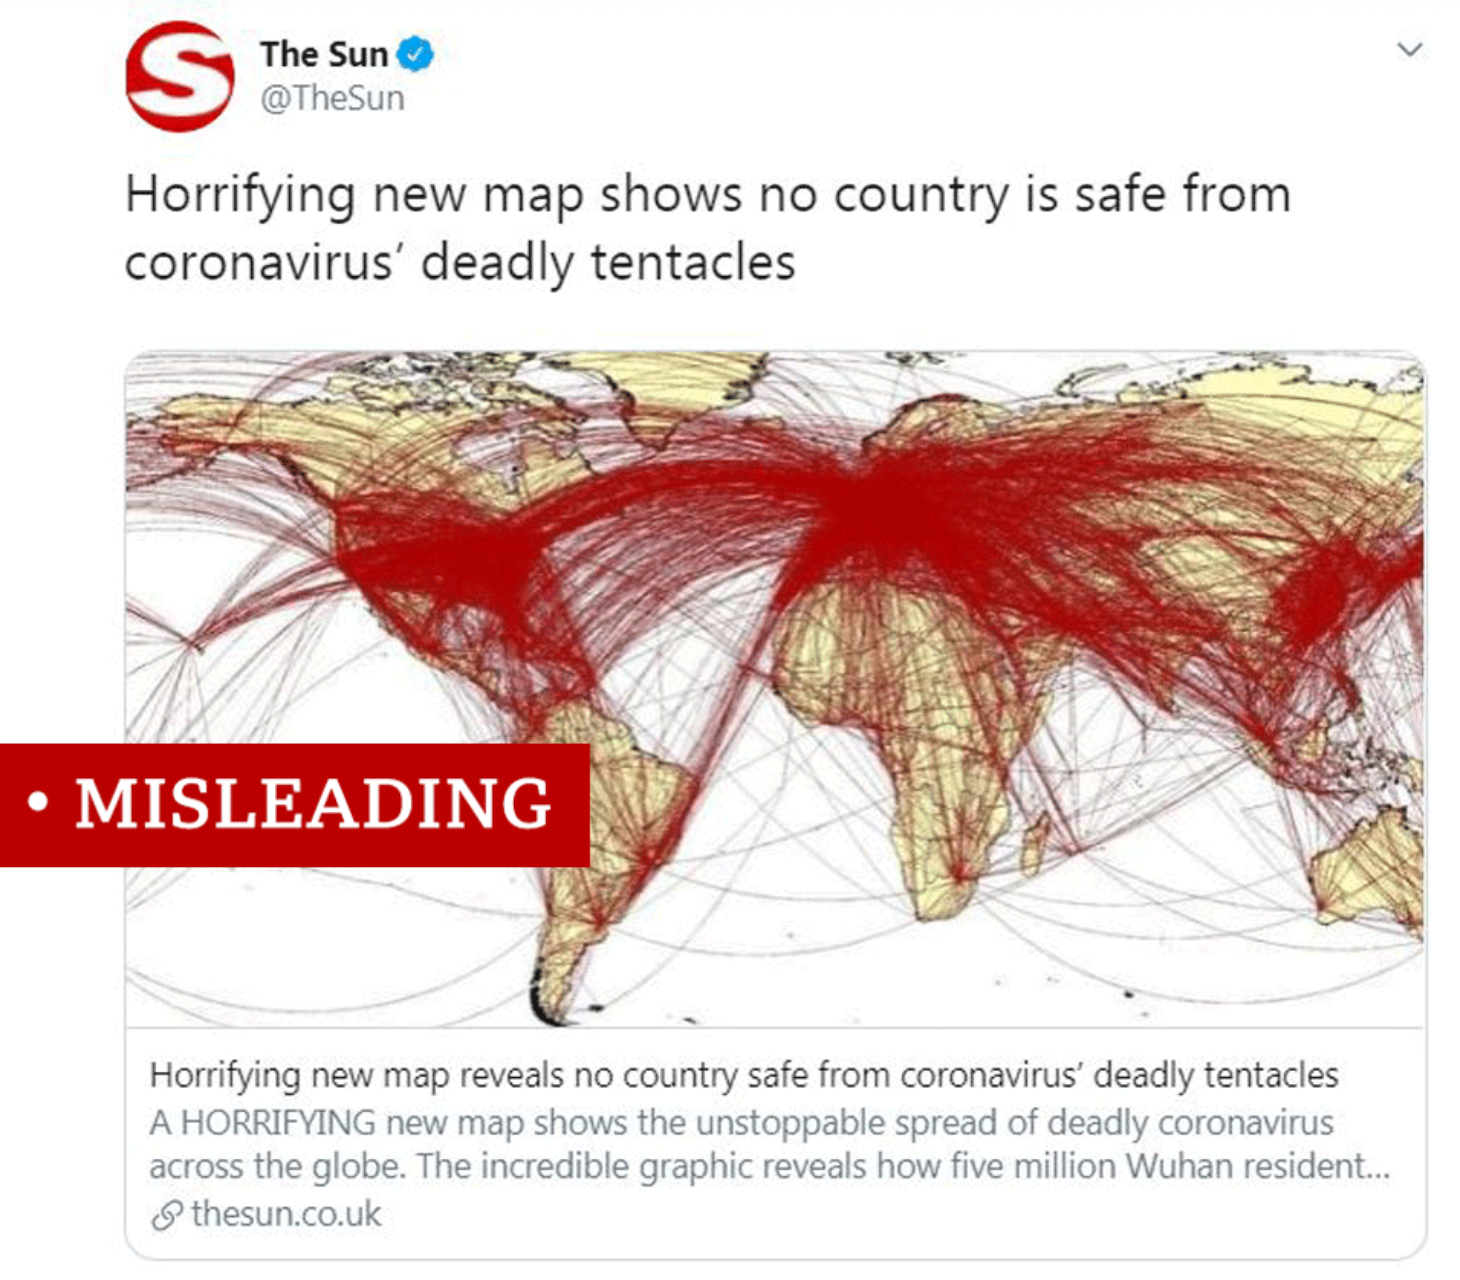
\includegraphics[scale=0.35]{COVID_but_not.png}
\end{center}

\end{frame}

%@@@@@@@@@@@@@@@@@@@@@@@@@@@@@@@@@@@@@@@@@@@@@@@@@
\begin{frame}
\frametitle{Chart Crime:}

\begin{center}
\huge \textbf{Underlying data is unrelated to graphic message.}
\end{center}

\end{frame}

%@@@@@@@@@@@@@@@@@@@@@@@@@@@@@@@@@@@@@@@@@@@@@@@@@
\begin{frame}
\frametitle{WTF?!}
\begin{center}
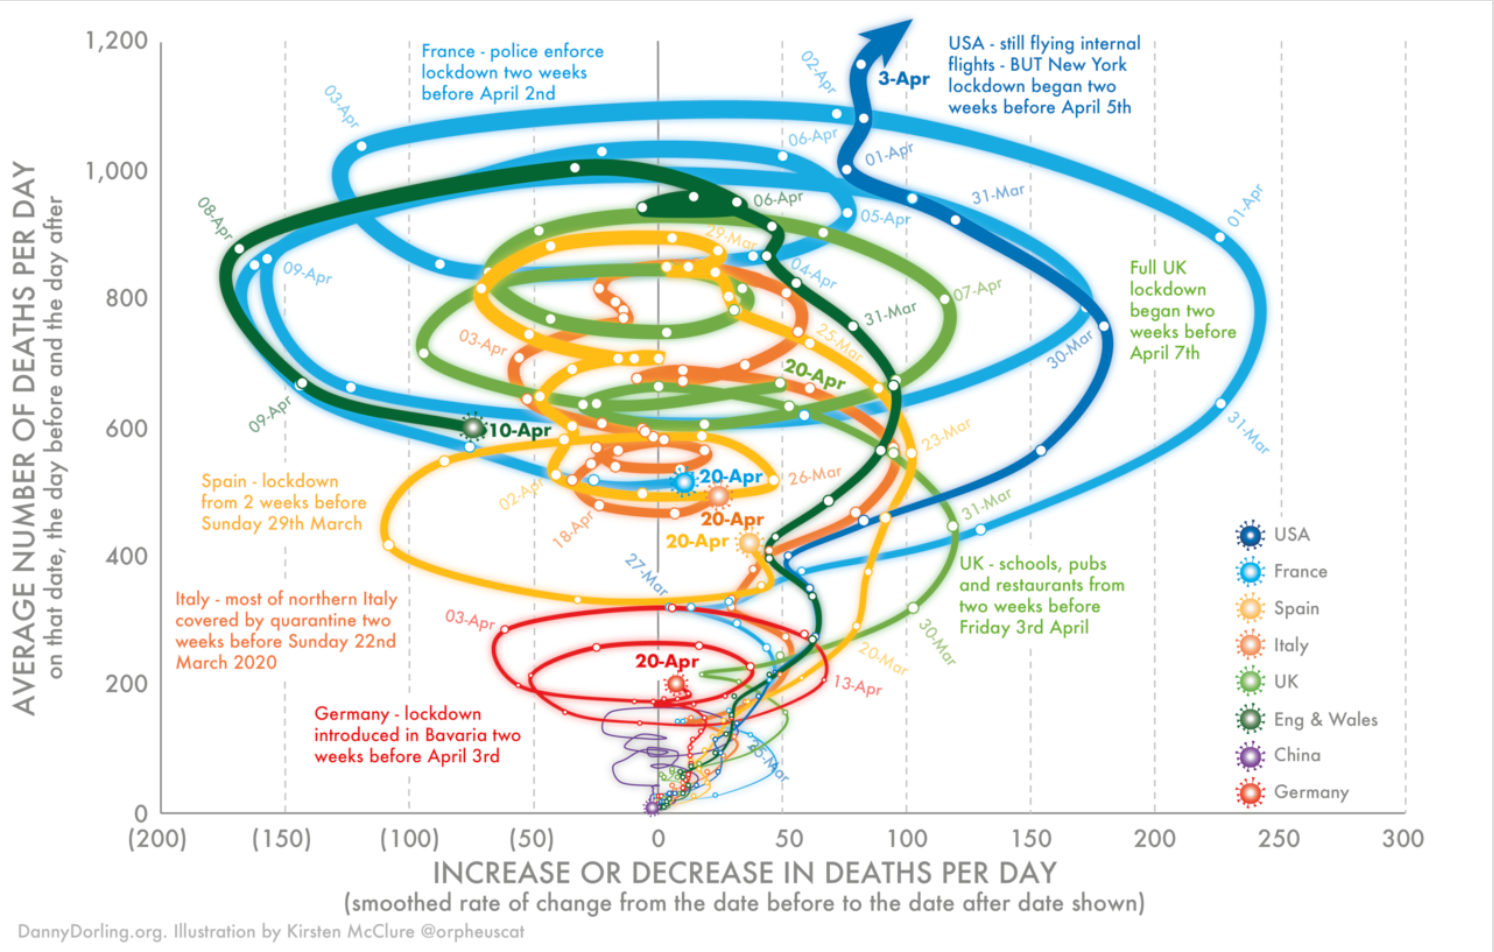
\includegraphics[scale=0.4]{crazy_chart.png}
\end{center}

\end{frame}

%@@@@@@@@@@@@@@@@@@@@@@@@@@@@@@@@@@@@@@@@@@@@@@@@@
\begin{frame}
\frametitle{Chart Crime:}

\begin{center}
\huge \textbf{No clear message, extremely difficult to interpret.}
\end{center}

\end{frame}

%@@@@@@@@@@@@@@@@@@@@@@@@@@@@@@@@@@@@@@@@@@@@@@@@@
\begin{frame}
\frametitle{Height Differences by Country}
\begin{center}
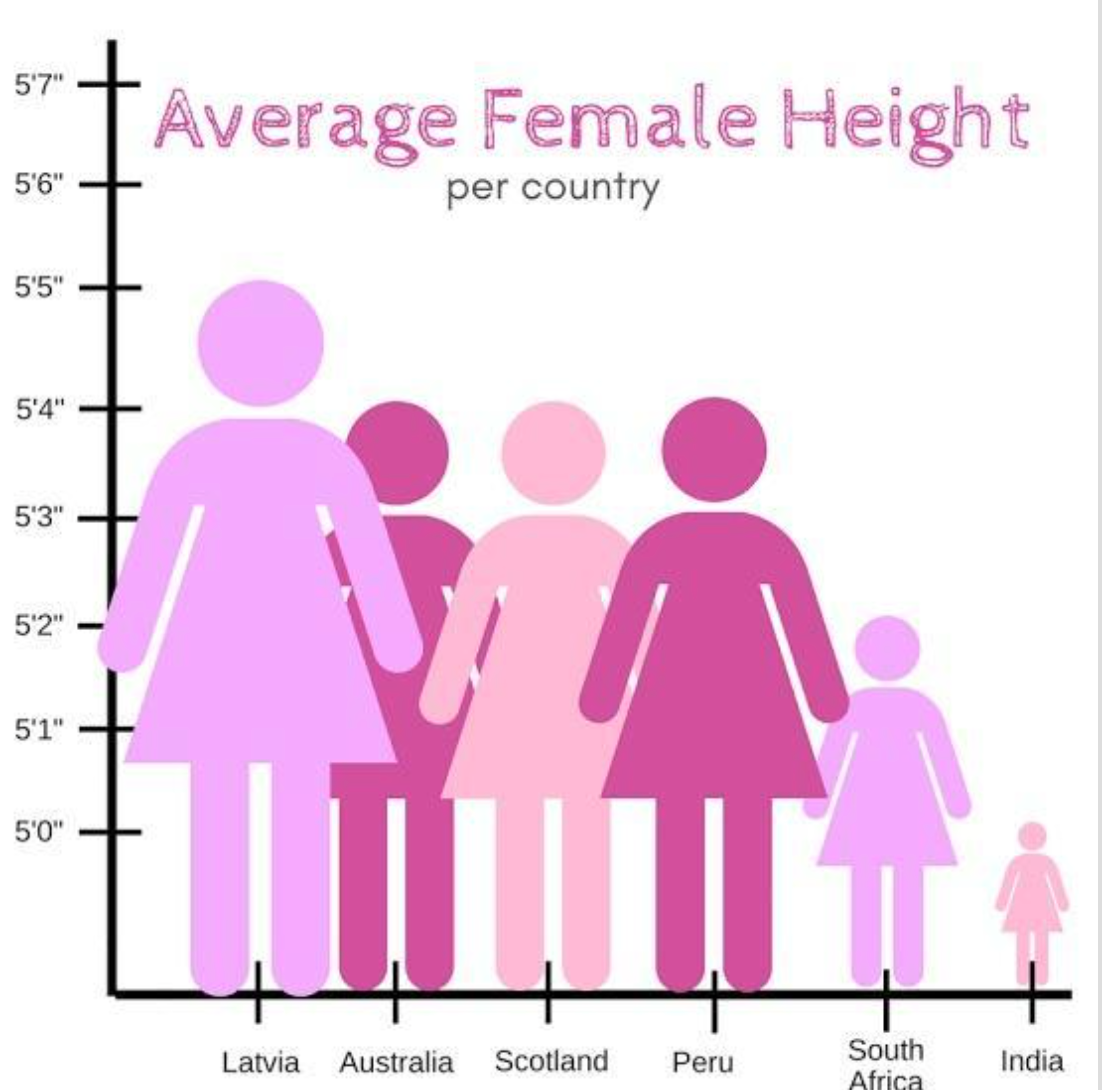
\includegraphics[scale=0.4]{giant_vs_small.png}
\end{center}

\end{frame}

%@@@@@@@@@@@@@@@@@@@@@@@@@@@@@@@@@@@@@@@@@@@@@@@@@
\begin{frame}
\frametitle{Chart Crime:}

\begin{center}
\huge \textbf{Truncated $y$-axis, misleading area comparison.}
\end{center}

\end{frame}

%@@@@@@@@@@@@@@@@@@@@@@@@@@@@@@@@@@@@@@@@@@@@@@@@@
\begin{frame}
\frametitle{Causality?}
\begin{center}
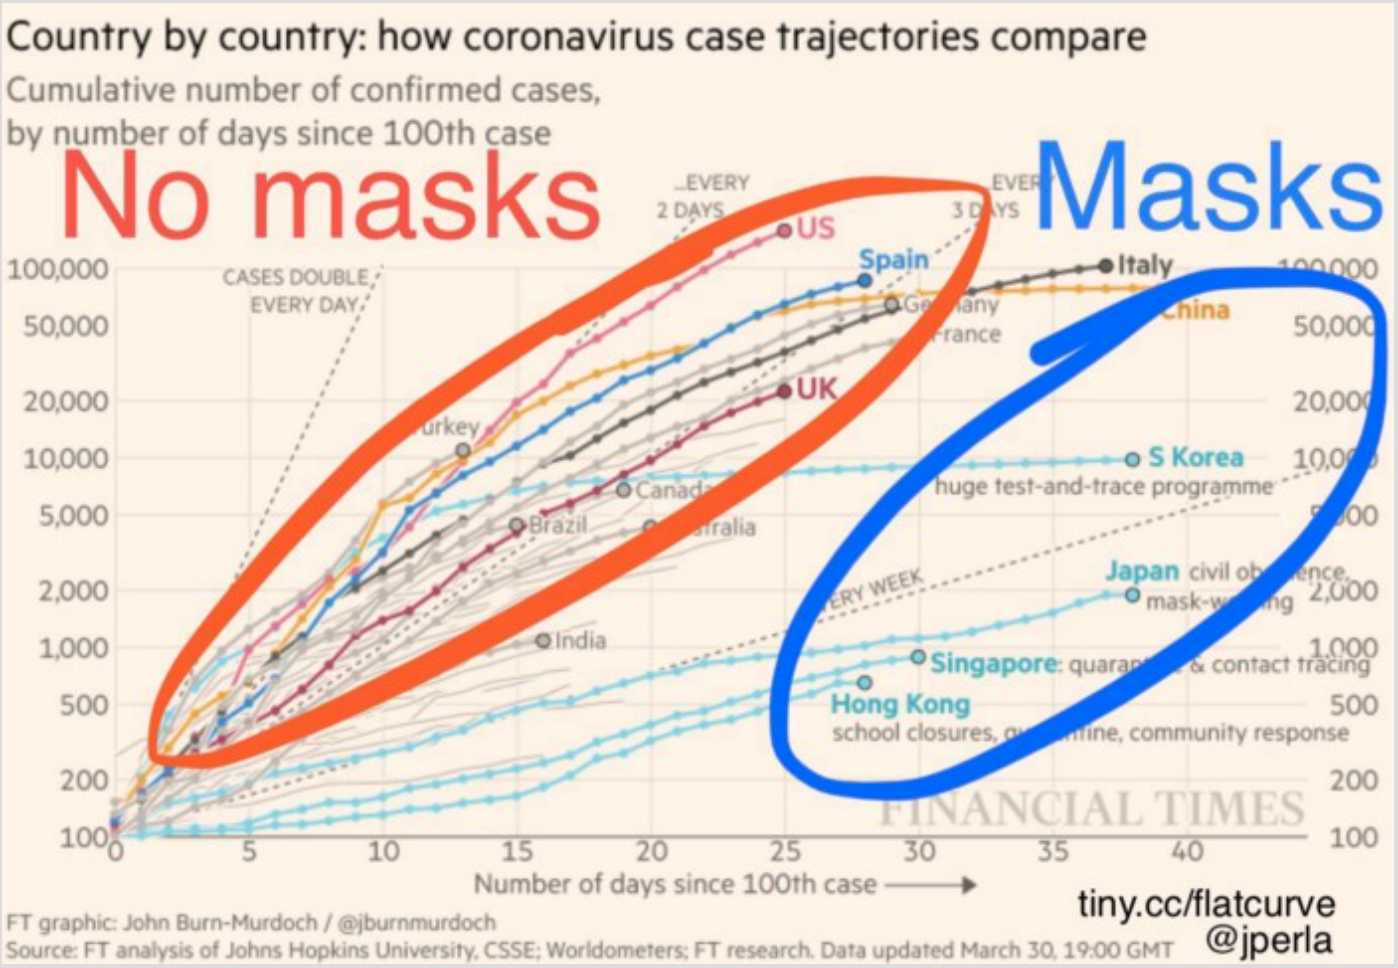
\includegraphics[scale=0.4]{misleading_causal_claim_1.png}
\end{center}

\end{frame}

%@@@@@@@@@@@@@@@@@@@@@@@@@@@@@@@@@@@@@@@@@@@@@@@@@
\begin{frame}
\frametitle{Causality?}
\begin{center}
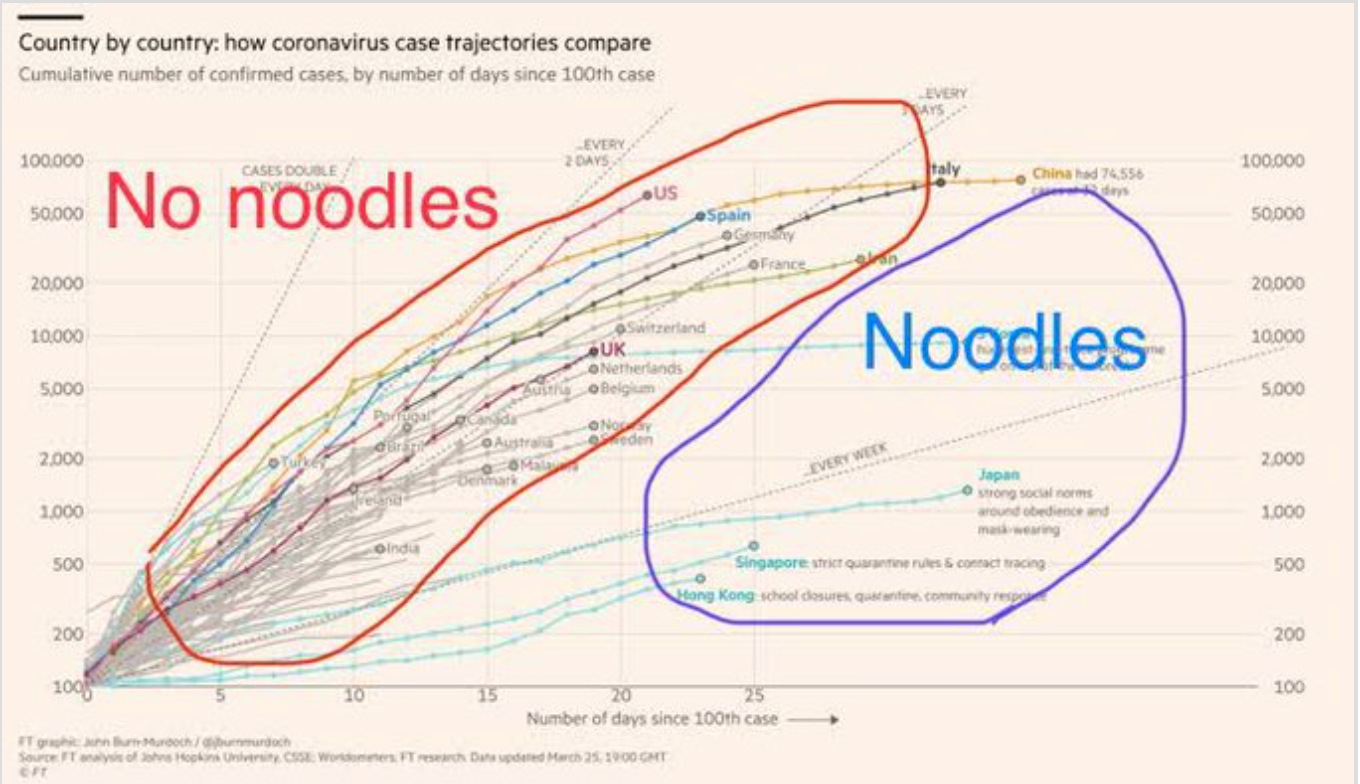
\includegraphics[scale=0.5]{misleading_causal_claim_2.png}
\end{center}

\end{frame}

%@@@@@@@@@@@@@@@@@@@@@@@@@@@@@@@@@@@@@@@@@@@@@@@@@
\begin{frame}
\frametitle{Chart Crime:}

\begin{center}
\huge \textbf{Asserting causality.}
\end{center}

\end{frame}

%@@@@@@@@@@@@@@@@@@@@@@@@@@@@@@@@@@@@@@@@@@@@@@@@@
\begin{frame}
\frametitle{Sino-Indian Diplomacy}
\begin{center}
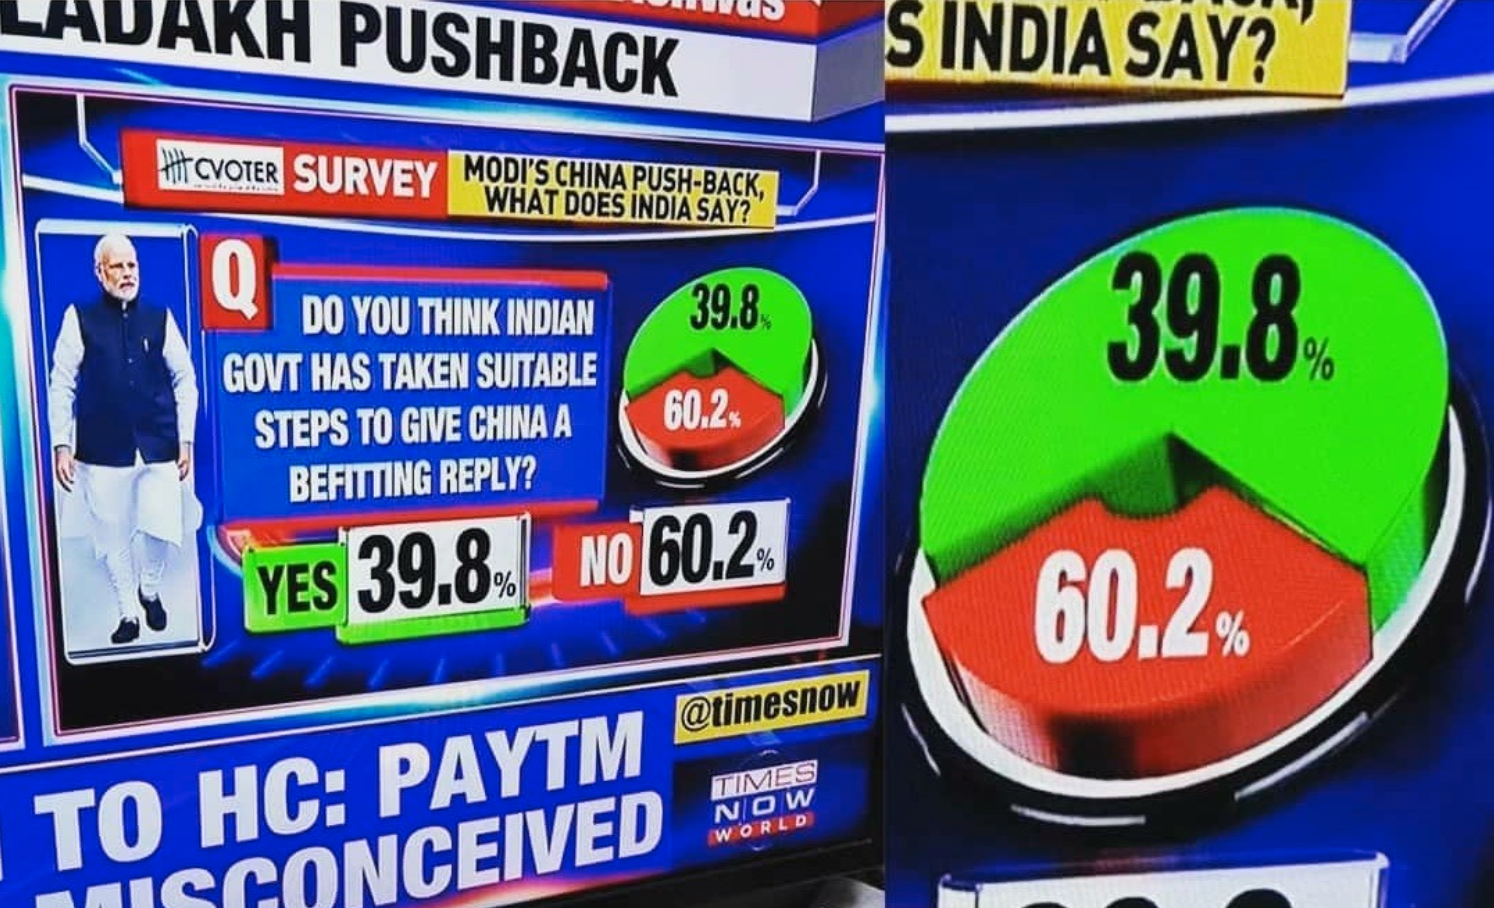
\includegraphics[scale=0.45]{misleading_pie_chart.png}
\end{center}

\end{frame}

%@@@@@@@@@@@@@@@@@@@@@@@@@@@@@@@@@@@@@@@@@@@@@@@@@
\begin{frame}
\frametitle{Chart Crime:}

\begin{center}
\huge \textbf{Misleading area comparison.}
\end{center}

\end{frame}

%@@@@@@@@@@@@@@@@@@@@@@@@@@@@@@@@@@@@@@@@@@@@@@@@@
\begin{frame}

\begin{center}
\Huge\textbf{Why should we care?}\\
\bigskip
\bigskip
\large A picture is worth a thousand table entries...\\
\end{center}

\end{frame}



\end{document}






